\documentclass[10pt]{ruthesis}
\special{papersize=8.5in,11in}

%\usepackage{natbib}
\usepackage[square,sort,comma,numbers]{natbib}

%\usepackage{color}
%\usepackage{aastex_hack,deluxetable} 
\usepackage{graphicx}
\usepackage{framed}
\usepackage{subcaption}

%\usepackage{rotating}
\usepackage{lscape,longtable}
\usepackage[utf8]{inputenc}
\usepackage{listings}

\lstset{
numberstyle=\small,
numbersep=8pt, 
frame = single, 
language=Python,
framexleftmargin=5pt}

\setlength{\unitlength}{1.0cm}

% Load packages; ambssymb is for extra fonts, such as blackboard
\usepackage{latexsym}
\usepackage{amsmath}
\usepackage{amssymb}
\usepackage{amsbsy}
\usepackage{verbatim} 

%\usepackage{color}
 

% Define Italic Sans Serif font (for tensors)
\DeclareMathAlphabet{\mathsfsl}{OT1}{cmss}{m}{sl}

%sectionbib option ensure sthat the bibliography is treated as a 
% section in your chapter, and not a new chapter.
%\usepackage[sectionbib,authoryear]{natbib} 
%\bibliographystyle{aj}

% Normal astronomical referencing is usually in the form (Smith
% 1999), this is to remove the extra comma in  (Smith, 1999).
%\bibstyle{aa}
\citestyle{aa}
\setcitestyle{square}

% to compile only the sections we are currently working on.
%\includeonly{warp1,summary,appendix_warpA,appendix_warpB}
%\includeonly{intro}

%to show notes on the margin, {\baselinestretch}{1} is because in 
% case double-space is used in the main text.
%\long\def\Notes#1{\marginpar{\renewcommand{\baselinestretch}{1} \tiny #1}}
%\long\def\Notes#1{\relax}
%\long\def\Ignore#1{\relax}
%\long\def\Comment#1{{\it\footnotesize #1}}

% The page number in Rutgers thesis format is so high up in the
% page that normal printers can not print it out! The following is to
% lower page numbers down a bit, so we can see them in a draft
% version to the committee members. Do NOT use this change in the
% FINAL version to be submitted to the Graduate School.
%\addtolength{\topmargin}{0.3cm}

\def\cha{{\em{Chandra}}}
\def\cxo{{\it{Chandra X-ray Observatory}}}
\def\ty{Tycho}
\def\e05{0509$-$67.5}
\def\n63a{N63A}
\def\casa{Cas A}
\def\p{PCA}
\def\C{Chapter~}
\def\einstein{{\em{Einstein}}}
\def\ginga{{\em{Ginga}}}

\hyphenation{iso-tropic para-meter para-meters}

%\draft
\setcounter{tocdepth}{1}

\begin{document}
\title{Towards Error Detection Test Framework for Molecular Dynamics Applications}
\author{Suvigya Tripathi}
\program{Electrical and Computer Engineering}
\director{Professor Shantenu Jha}
\approvals{3}
\submissionyear{2016}
\submissionmonth{October} 

\abstract{
The reliability of a fully developed and error-free software is critical, since it determines a software's credibility and user satisfaction in the application. A major challenge in the field of testing is to bridge the gap between the customer requirements and the actual outcome of the software. There are several tools in the field of chemical sciences for Molecular Dynamics (MD) simulations. The EnsembleMD Toolkit is a Python framework for developing MD applications providing an abstraction that enables the efficient and dynamic usage of High Performance Computing (HPC), simultaneously hiding the complexity of allocation and execution in the underlying layers. 

The EnsembleMD toolkit facilitates a simple framework for MD applications, but it lacks the feature of testing the functionality during its software development cycle (SDC). Checking the errors and faults at all stages of the SDC, namely, development, deployment on supercomputers and run-time, is crucial to ensure the proper functioning of the scientific tools and applications.

The frequent changes in the system configuration of supercomputers imposes the necessity of a platform which can provide sanity check on all of the components and modules. Hence, to address these requirements, we developed a Testing Framework. The framework has three primary design components: (1) Support of testing APIs of the toolkit during development, (2) Support for testing of faults during their deployment on supercomputers and (3) Support for logging the run-time exceptions and errors. This bench enables the developers of various scientific tools viz. EnsembleMD toolkit, Amber, CoCo etc to easily and scalably debug the issues faced by the end users. 
}

\beforepreface

\acknowledgements{
First and foremost, I would like express my heartfelt gratitude to Dr. Shantenu Jha for having faith in me and giving me the opportunity to work on this project. I am very thankful to Dr. Jha for his encouragement and support through all the years of my grad school, Without his guidance it would not have been possible to finish this thesis. I would also like to thank Dr. Jha for the training, advice and motivation that kept me focused during the course of this project which helped me to overcome both professional and personal challenges. \newline\newline
Besides my advisor, I would like to thank the rest of my thesis committee
for their encouragement, insightful comments, and challenging questions.\newline\newline
I would like to thank Vivek, Antons and all members of the RADICAL team for their support and involvement in the development of this project. Without their passionate participation and input, the project could not have been successfully 
completed. I am also grateful to the ExTASY team for their continuous feedback and support during the entire course of this thesis. I thank XSEDE and TACC for resources I used. I would also like to thank Rutgers University for providing me an opportunity to study here and nurture my career and future. \newline\newline
Finally, I must express my very profound gratitude to my parents for providing me with unfailing support and continuous encouragement throughout the process of researching and writing this thesis. Love to Shubhangini, Gayatri and Ankit for your support. This accomplishment would not have been possible without them. Thank you!
}

\dedication{
\begin{center}
{\em Dedicated to family and friends} \\
\end{center}
}

\figurespage
\tablespage

\afterpreface

%%Chapter 1
\chapter{Introduction}
\section{Motivation}
 As supercomputers and High Processing Cluster increase in size and complexity, system failures have become inevitable \cite{ref7}. These failures have a great impact on the available computing resources. Around 1.53\% of the total applications failed during the initial 518 production days of Blue Waters contributing to 9\% of the total production node hours \cite{ref6}. These errors are reported not only because of the system failures, but might also occur due to an application or software bug. A software bug is an error in the programming and coding of the application that might cause it to malfunction. These bugs often have a major impact on cost, money or time. Software failure can lead to serious consequences in safety critical and normal applications. Software testing is defined as a formal process in which a software unit, several integrated software units, or an entire package, are examined by running the programs on a computer with various inputs and expected outputs. It is the primary method for assuring high quality, error free software.  All the associated tests are expected to generate results similar to the results generated during actual execution. Testing plays a central role in quality assurance of any application. In a software development cycle, testing is paramount during the development and pre-delivery phases of any software. 
 
 A Testing framework is essential for error control that can be categorized into error detection and error handling and correction. Error detection is the most important stage for developing reliable and highly dependable computing as it deals with the detection of error generated due to software defects or hardware failures. The error report generated by the error detection phase can be used by the developers to handle and rectify the defects. Testing is a continuous cycle of error control mechanisms which operates until the software has negligible defects or the error lies within the acceptance criteria. A plethora of applications has been developed to perform Molecular Dynamics simulations and analysis. Many of these applications in the field of molecular sciences use ensemble-based methods as their basis to make scientific progress. EnsembleMD toolkit is one such toolkit that provides abstraction layer for executing various scientific simulations where multiple computational execution units form a part of an ensemble referred to as tasks. 

Traditionally, developers of EnsembleMD toolkit had to backtrace all of the logs from supercomputers, logs from Radical-Pilot and EnsembleMD to debug any failure or exception issue. Job submission and execution on remote supercomputers may fail due to various factors, viz. failure due to bugs in source code, wrong kernel inputs, exception if connection to database fails, failed job submission or the modules and configurations specific to the kernel and supercomputer is loaded incorrectly. This generally leads to multiple drawbacks. The major drawback is that it isolates the error and exception causing component. It is cumbersome to debug innumerable logs and investigate the failures and faults. The failures and errors reported by the users using hardware or compilers that have not been extensively tested by the developers can cause loss of precious time and developers need to put efforts to identify and isolate the errors \cite{ref16}. As discussed earlier, detecting errors is crucial in error control mechanism of any test framework, aforementioned problem to detect errors in molecular dynamic application serves as the motivation for this thesis. The developers and the users of EnsembleMD toolkit and other scientific toolkits would benefit largely from this testing framework that encapsulates the following:

\begin{itemize}
	\item Automate the cumbersome process of debugging and isolating errors and exceptions.
	\item Support a testing bench to ensure the expected functionality of all the APIs in the toolkit.
	\item Eliminate manual efforts to check for proper configurations required by supercomputers to execute different kernels.
	\item Possess capability to execute all the tests automatically whenever functionality of the toolkit is added or modified. 
	%\item Generate an automated detailed report for analysis. 
\end{itemize} 

\section{Objective}
The main objective of this thesis is to develop a test framework to enable the validation of open source tools like the EnsembleMD toolkit and RepEx and to test the proper functioning of all the APIs. Furthermore, the aim is also to develop a framework that tests the deployment and run-time errors which may occur while executing scientific tools on remote supercomputers. Another objective is to analyze the requirements and develop an automated test bench for the developers with the following capabilities:

\begin{itemize}
    \item Enable a test bench to ensure that the development code meets its design.
	\item Enable remote supercomputer configuration and environment checking at the time of deployment.
	\item Enable a framework to detect the run-time faults and errors by mining the logs generated on the supercomputers at the time of execution of an application.
	\item Ensure that the toolkit behaves as expected and provides interoperability to enable execution over multiple heterogeneous distributed computing infrastructure.
\end{itemize}
   
\section{Structure of the Thesis}
After discussing the motivation and objectives for this thesis in Chapter 1, we will discuss the various research and related works in Chapter 2 followed by a discussion on the background of the Radical EnsembleMD toolkit and Radical RepEx framework in Chapter 3. In Chapter 4, we will explore the testing infrastructure, its significance and testing framework design for the toolkits. In Chapter 5, we will discuss the development level testing of EnsembleMD and RepEx. Development level testing includes unit testing and end to end testing to ensure a bug-free tool. SATLite, a standalone testing tool to test deployment and run-time errors will be discussed in Chapter 6. Chapter 7 illustrates the automated testing harness and integration with the Jenkins Continuous Integration (CI) server in depth along with the testing results. In Chapter 8, we arrive at the conclusion and discuss the foundations this thesis lays for future work. 

%Chapter 2
\chapter{Related Work}
A large percentage of today's high computing performance and resources are wasted due to various
failures. These failures significantly affect the capacity of HPC clusters and the logs generated by the clusters are abundant in number and mining these logs to detect the error is very cumbersome.
Unfortunately, designing an ideal fault-free high computing resources is unfeasible. However, there is always a trade-off between high processing computing and fault-free resources. We can design a highly dependable system by having a solid understanding of its failures and characteristics \cite{ref8}. 


Current research in the field of testing the faults and errors generated in supercomputers and a large number of mining tools have been developed to study and analyze the logs. Martino et al.'s \cite{ref6} study on the impact of system failures on the Blue Waters had shown the effect on the available node hours. To study and analyze these failures, they developed \textit{LogDiver} which is a tool to automate the system log data processing. \textit{LogDiver} handles large amounts of textual data extracted from the system and application level logs and decodes the specific types of events and exit codes. Their study shows that probability of application failures due to system failures is just 0.162.

Chuah et al. \cite{ref9} studied the root causes for the failures using system logs of the Ranger supercomputer at the Texas Advanced Computing Center (TACC). \textit{FDig}, a diagnostic tool had been developed to extract the log entries as structured message templates to analyze the faults. \textit{FDig} detects the frequency of the specific errors by extracting the error template messages from the stored system logs and supports system administrators in the fault diagnostic processes. The research and development of the fault tolerant system is continuous. 

The current ongoing research primarily focuses on providing fault tolerance strategies with an objective to minimize the fault and failure effects on system resources. Gainaru et al. \cite{ref12} extensively exploited the concepts of data mining techniques to determine system errors from the logs generated by Blue Gene/L machine. They have also used the signal analysis concepts to shape the normal behavior of the system events. Their study was focused on the normal behavior of a system and the effects of faults on the system.

According to \cite{ref6}, \cite{ref9}, \cite{ref13}, console logs are a primary source of information about the condition of a cluster or HPC system. These error logs help system administrators to analyze the causes of system failures. Gurumdimma et al. \cite{ref13} developed a tool to increase the time window by around 50 minutes between the first event of error message in the log file and the time of ensuing of the failure. This increase in the time window gives sufficient time to the administrators to save the state of the running applications, hence, saving large execution time. The development of their tool had basis on anomalies in the resource usage logs and mining of error logs for Ranger Supercomputer from TACC. Similar research has been conducted by Zheng et al. \cite{ref15} to develop FTC-Charm++, a fault-tolerant runtime based scheme for fast and scalable recovery of the applications on the HPC clusters. 

A study by Oliner et al. \cite{ref14} on the system logs from five supercomputers, namely, Blue Gene/L, Red Storm, Thunderbird, Spirit and Liberty which analyzed failure alerts and actual failure shows that a large number of alerts are generated due to hardware issues, but most of the system failures are due the software issues. A possible explanation of system failures is due to software upgrades. The applications running on these resources might not be compatible with the software upgrades and hence leads to their failure. 

Analyzing the system logs forms the basis of various testing tools for the HPC clusters. Chen et al. \cite{ref10} have adopted Hidden Markov Model (HMM) \cite{ref11} along with the frequency analysis to predict job residual times. It is beneficial for the job scheduler to predict the status of every job for proper resource management. Chen and group's approach can predict 75\% of the job's running times with an error of less than 200 seconds.  

All of the novel approaches discussed earlier in this section describes the strategies to anatomize the system logs and error log files to detect the system errors. These studies however show how to combat the effect of system failures and predict them to minimize the errors and faults. There is a window of opportunity for further improvement in the efficiency of resources if we can minimize the errors during application job submission. The large sector of computing resources is used by Molecular Dynamics simulations. These applications are responsible for complex simulation and analysis of various molecular structures. There is always a major cost associated if these molecular dynamics applications fail. The scientific simulation workflows such as Amber, CoCo, etc. are the major tools in the field of molecular dynamics domain. These workflows serve as input to various tools such as Radical EnsembleMD and Radical Pilot. With the advancement in these workflows, it is highly possible to have software bugs. In order to minimize the effect of application failures due to source code bugs, improper environment loading or transferring incorrect input files, we have developed a testing tool, \textit{Simple Application Testing Lite (SATLite)} to detect the application deployment level and run-time errors. The developers of scientific workflows can directly check for errors while their software is still under development, before releasing it to their user base. The dependency of these scientific simulation packages on different operating systems and HPC clusters remains undetected unless a full compilation is made, and errors with``make clean" \cite{ref16} can build successfully on a developer's machine, but can fail on user machines. Betz et al. \cite{ref16} have discussed the effect of application bugs with respect to AMBER development in depth. Since, major research in the field of HPC fault-tolerance system uses different logs, we have also used system and console log mining approach for designing our tool. 



%%Chapter 3
\chapter{Background of Radical Tools}
\label{chap:background}
Molecular Dynamics (MD) simulations is a key method to study protein structures, gene finding, sequence analysis etc. These simulations are highly important in the field of drug design and drug discovery to study active molecules and protein interaction sites \cite{ref1}. The gene sequence and protein structures are highly important in the detection of diseases, hence, the analysis of these components are highly critical and requires high computing processing. Due to the high complexity of the molecule structure, high performance and parallel computing provides a substantial improvement in time taken for various calculations. The High performance computing (HPC) approach helps to minimize the number of target drugs that is required to be tested by expensive and time-consuming synthesis and laboratory experiments [1]. There are several tools that provides interface for the MD simulations. ExTASY tools such as Amber, CoCo, Gromacs and LSDMap are the scientific tools for MD simulations. Radical-EnsembleMD toolkit (EnMDTK) and RepEx provides an interface for the resource handling and execution of the former tools on the remote HPC clusters. This chapter deals with the background discussion of the toolkit whose testing framework has been developed.

\section{About EnsembleMD Toolkit}
EnsembleMD Toolkit is a python based framework for developing, simulating and executing molecular science applications comprising of ensembles of simulations. This toolkit is designed to address the issues of decoupling of tasks, heterogeneity across them and the dependency between them \cite{ref3}, \cite{site1}. This provides a tool for MD applications which efficiently decouples the details of execution units and manages their submission on the remote machines. It provides abstraction to the users, hiding the complexity of the mechanism of job submission, execution and data transfer. EnsembleMD Toolkit provides a set of explicit, predefined patterns that are found in ensemble-based MD workflows \cite{ref2}, \cite{ref3}, \cite{site1} . Users have an advantage of picking up the patterns which represents their application and populate it with MD engines viz. Amber, Coco, Gromacs or LSDmap, represented by 'kernel' in the tool. Even though traditional tools gave complete control to users to manage MD applications, the major drawback was that the user was required to have knowledge of load transfer, job submission or data flow control. Users were required to explicitly undergo these cumbersome tasks of resource allocation, job submission and execution. In case of EnMDTK, this complexity is hidden from the user, hence it provides a simple yet efficient way to execute their application.

\subsection{Design of EnsembleMD Toolkit}
Ensemble-based applications comprises of tasks that may vary in the type of coupling between them or the amount of information transferred between them. Each of the tasks, with or without coupling, have different computational requirements \cite{ref2}, \cite{ref3}. EnsembleMD Toolkit was designed with an aim to provide a framework for multiple tasks with varying coupling levels on different HPC clusters. The modular design of the tool serves as a building block to make MD application execution flexible and scalable.

Figure \ref{fig:enmd_arch} \cite{site1} shows the architecture of EnsembleMD toolkit. As depicted in the figure, execution of any MD application takes place in five steps, namely:

\begin{itemize}
	\item Pick execution pattern representing the application.
	\item Define kernel plug-in for various stages of the pattern.
	\item Resource handler creation and request for resource submission.
	\item Call Execution plug-in to bind pattern and kernel plug-in and run job on remote resource.
	\item After successful execution, de-allocate the resources and user gets back the control.
\end{itemize}

\begin{figure}
  \centering
  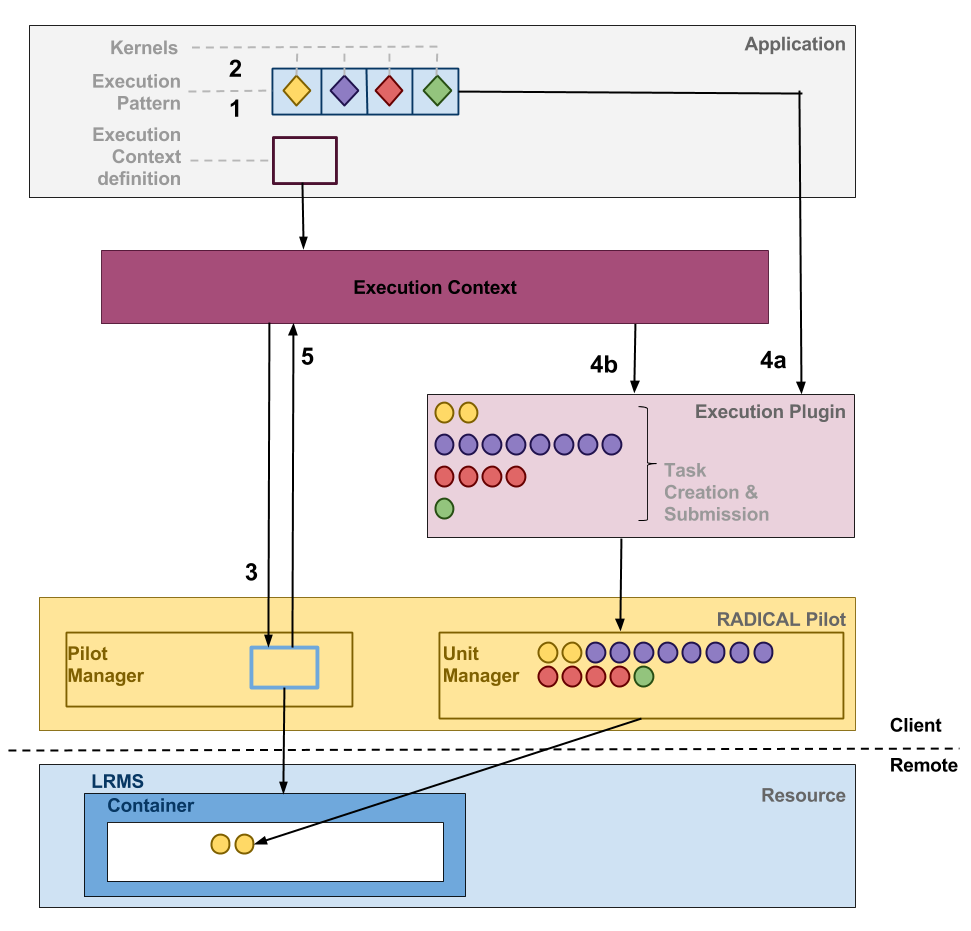
\includegraphics[width=13cm,height=13cm]{enmdtk_arch.png}
  \hbox{\small\itshape Credit: EnsembleMD toolkit architecture document} \cite{site1}
  \caption{Architecture of EnsembleMD Tool}
  \label{fig:enmd_arch}
\end{figure}

\section{EnsembleMD Toolkit Components}
As discussed in the above steps, EnsembleMD tool architecture comprises of four basic components showcasing the heterogeneous property of the tool that are described in details in subsequent subsections.

\subsection{Execution Patterns}
MD application control flow can be categorized into a few repeating types. EnsembleMD tool exploits this characteristic to define a high level object describing the control flow or {\em``what to do"} at different stages. An execution pattern represented by \textbf{{1}} in figure \ref{fig:enmd_arch} describes a parameterized container which can hold and execute ensembles. 

\subsection{Kernel Plugins}
A Kernel plug-in represented by \textbf{{2}} in figure \ref{fig:enmd_arch} is an object that abstracts a computational task in this toolkit. It represents the instantiation of a specific science tool along with the required software environment. Kernel hide tool-specific peculiarities across different clusters as well as differences between the interfaces of the various MD tools to the extent possible. 

\subsection{Resource Handler}
The resource handler represented by \textbf{{3}} in figure \ref{fig:enmd_arch} manages the resources for various job submission and execution on HPC cluster. It provides the following methods:
\begin{itemize}
	\item Allocate resource
	\item Run execution pattern on allocated resource
	\item Deallocate resource
\end{itemize}

\subsection{Execution Plugin}
The execution plugin represented by \textbf{{4}} in figure \ref{fig:enmd_arch} is an internal component of the toolkit managing the execution of the execution patterns. This layer binds the execution pattern with the kernel plugins, hence, generating the executable units which are forwarded to the underlying runtime system along with the resource details. This plugin decouples the execution plugin into an executable plugin enhancing the runtime optimization of various parameters, viz. time to completion, throughput etc. 
As we have discussed earlier, the EnsembleMD toolkit is an abstraction tool which hides the complexity within the underlying layers and only exposes the plugins to the users. Execution pattern, kernel plugin and resource handlers are exposed to the users, whereas execution plugin manages the underlying complexity of decoupling the tasks, binding patterns and plugins, job submission, job execution and data transfer. This hidden complexity is addressed by the Radical-Pilot layer, which is the most crucial component of the toolkit architecture. 

\subsection{Radical Pilot}
Radical-Pilot is a Pilot job framework which allows users to run a large number of computational tasks simultaneously on one or more different distributed systems such as remote HPC clusters. A Pilot-job is responsible for acquiring resources necessary to execute the computational units on the HPC cluster. The Pilot-job submits the jobs or the units to the system's batch queue. These pilot jobs are the containers that carries the number of tasks or executable within itself. Once these pilot jobs becomes active, it can run sub-jobs directly, by eliminating the need to submit a separate job for each executable differently and hence, reducing time-to-completion. Radical Pilot provides task-level parallelism, by executing a large number of tasks concurrently on the HPC cluster. In other words, typically in absence of any such job submission framework, if the application has a complex workflow that requires several tasks to be executed, each task or job is required to be submitted individually with the queue wait time. This call for a resource management framework can effectively submit parallel jobs, hence, enhancing the effective use of the available resources.

\begin{comment}
\subsection{Architecture: Radical-Pilot}
Figure \ref{fig:pilot_arch} shows the architecture of Radical-Pilot. Application layer consists of actual application which are defined in terms of Compute Units. Compute units can be considered as self-contained executable part of the application. Radical-Pilot components provide task level abstraction using Compute units and decoupling of workloads. It also provides interoperability using underlying SAGA (Simple API for Grid Applications) layer. Radical-Pilot Agents (RP Agent) runs on the remote machine and launches compute units or executable using requested cores.

\begin{figure}
  \centering
  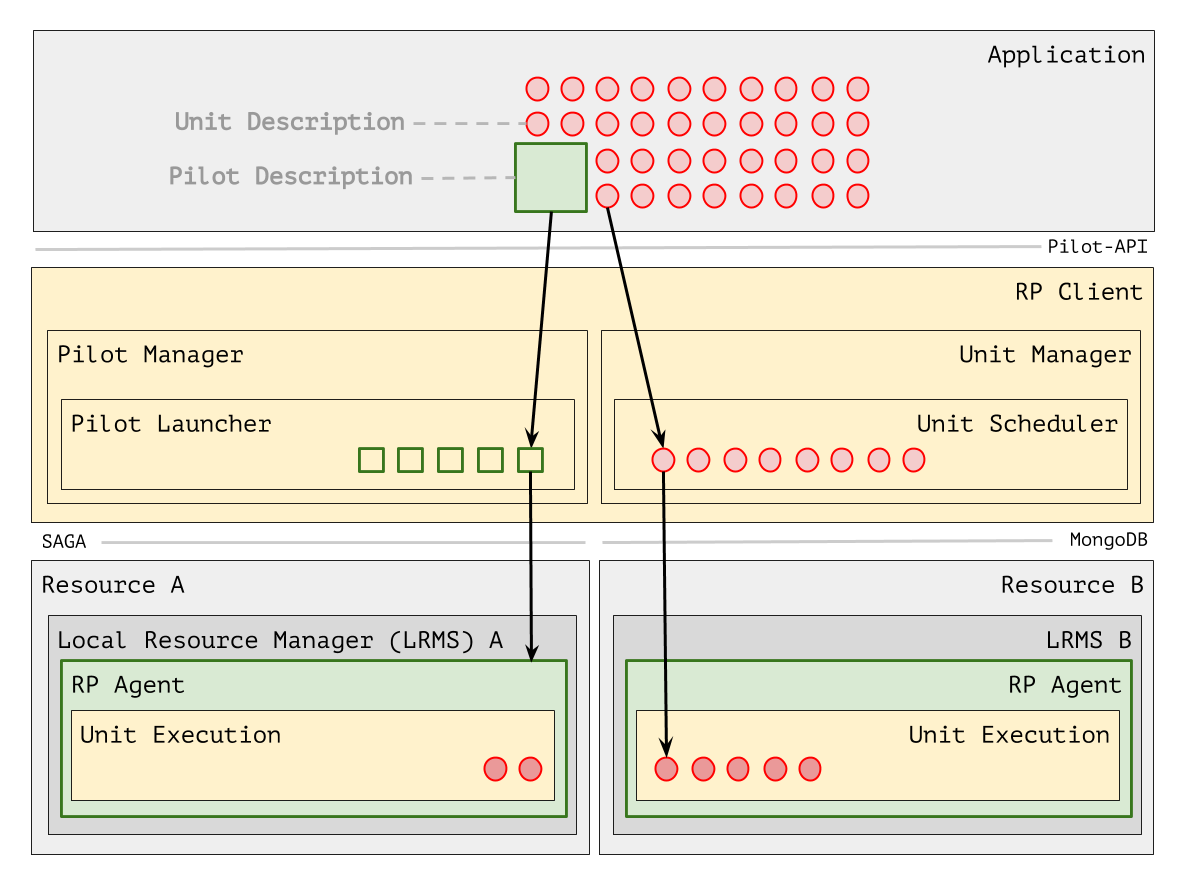
\includegraphics[width=13cm,height=10cm]{pilot_arch.png}
  \hbox{\small\itshape Credit: Radical Pilot architecture document}
  \caption{Architecture of Radical Pilot}
  \label{fig:pilot_arch}
\end{figure}

\subsection{Radical-Pilot Components}
\begin{itemize}
	\item \textbf{Pilot:} Pilot is an empty container that gets submitted on remote HPC cluster. These get submitted into the remote machine's queuing system and acquires the resources.
	\item \textbf{Compute Unit:} A compute unit is a self-contained executable part of the specific application.
	\item \textbf{Pilot Manager:} Pilot Manager is responsible for the resource management and interaction between the pilots. it also determines how to group compute units before deploying them on to the remote machines.
	\item \textbf{Unit Manager:} Unit manager maps each compute units to the pilots. It comprises of scheduler which provides algorithm for this mapping.
	\item \textbf{MongoDB:} MongoDB is the interface for communication between RP application and created pilots. Whenever execution starts, pilot connects to the database and seeks the compute units. Also, pilot pushes the intermediate data, final data or other information on the database.
	\item \textbf{Pilot Agent:} Pilot job is the container job on the remote machine side. It manages the scheduling, submission and execution of the compute units on the remote resources with specified system requirements.
\end{itemize}

\subsection{Radical-Pilot Operation}
The application submits a pilot with specific size to the remote HPC cluster along with active time duration. After the successful submission of the pilot, application is defined in terms of compute units which are submitted to the unit manager. The sequence of execution of various executable components of the application is also managed by the unit manager. It consists of a scheduler which maps compute units to the pilots. Unit manager is also responsible for staging any input required during the compute unit execution either from the remote resource or the local machine. These Compute Units are updated in the MongoDB database. The stored Compute Units apart from the executable, also consists of the shell script which sets up the environment, loads the required modules for execution and input data \cite{site3}, \cite{ref22}.

The Pilot Agents after becoming active on the remote resource, pulls these Compute Units from the database and schedules or queues them on the requested resource. Radical Pilot Agent updates every stage starting from Pilot submission to Compute Unit execution into the database. It also synchronizes with Unit Manager and polls more Compute Units, if available. Pilot Agent manages the output data from the Compute Units back to the local machine. On successful execution and termination of the application, the Pilot on the remote machine is canceled.
\end{comment}

\section{Patterns in EnsembleMD Toolkit}
As discussed earlier, the work flow in molecular sciences applications can be categorized into repeating types, motivating the developers to create an abstraction layer called ``patterns." EnsembleMD toolkit has four patterns which envelopes almost all the MD applications. The next few subsections will discuss the different types of ``patterns."

\subsection{Pipeline}
A pipeline pattern consists of a sequence of executable stages. The EnsembleMD toolkit pipeline pattern, as shown in figure \ref{fig:pipeline} \cite{site1}, is the primary pattern that consists of a container of independent tasks that contains heterogeneous workloads. The data flow and control mechanism is always unidirectional and follows a linear pattern. Each pipeline stage might have dependency from previous stage and executes independently. 
\begin{figure}
  \centering
  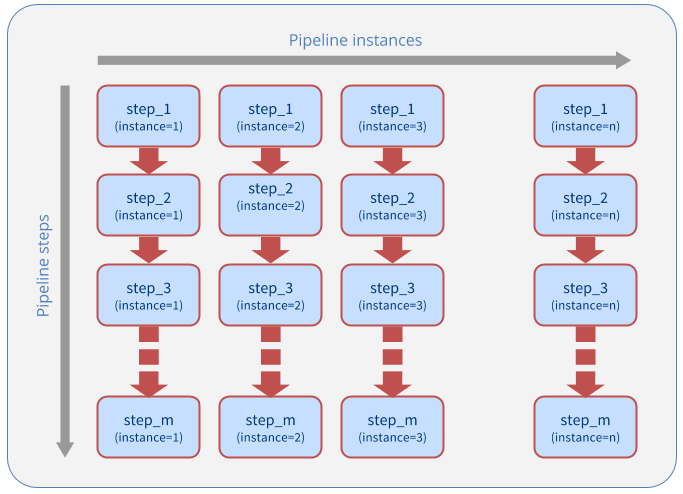
\includegraphics[width=12cm,height=8cm]{pipeline_pattern.png}
  \hbox{\small\itshape Credit: EnsembleMD toolkit architecture document \cite{site1}}
  \caption{Pipeline Pattern}
  \label{fig:pipeline}
\end{figure}

\subsection{AllPairs}
The All-pairs problem is stated as:
All-Pairs(set A, set B, function F) returns a matrix M which is composed by comparing all elements of set A to all elements of set B using the function F. Otherwise
stated as, M[i,j] = F(A[i],B[j])[12]. A pictorial representation is given in Figure \ref{fig:allpairs}
\begin{figure}
  \centering
  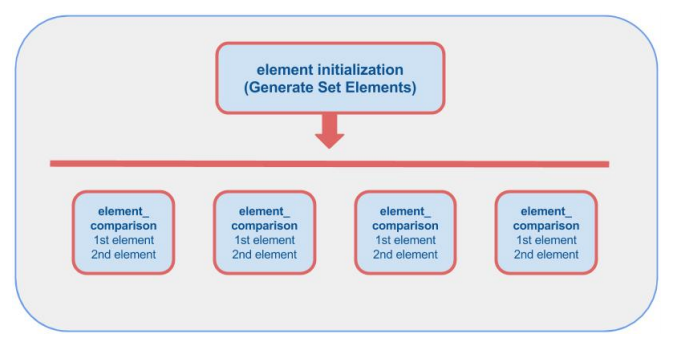
\includegraphics[width=13cm,height=7cm]{allpairs.png}
  \hbox{\small\itshape Credit: EnsembleMD toolkit architecture document \cite{site1}}
  \caption{Allpairs Pattern}
  \label{fig:allpairs}
\end{figure}

\subsection{Replica Exchange}

Replica Exchange pattern is a generalization of Replica Exchange Molecular Dynamics (REMD) conformational algorithm \cite{ref4} and is divided into two stages, namely: Simulation stage and Execution stage. The Replica Exchange pattern starts with each replica propagating simulation phase independently, followed by the exchange phase where exchange of thermodynamic patterns takes place. This exchange is determined on the basis of the results of simulation phase. Figure \ref{fig:repex1} \cite{site1} depicts execution of simulation and exchange phase with various degree of concurrency depending on the number of iterations.

\begin{figure}
  \centering
  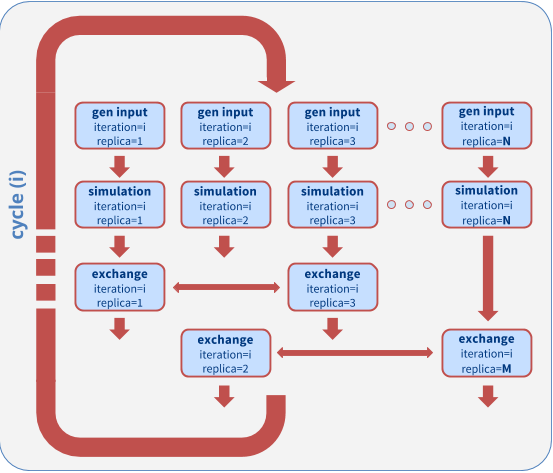
\includegraphics[width=12cm,height=9cm]{repex.png}
  \hbox{\small\itshape Credit: EnsembleMD toolkit architecture document \cite{site1}}
  \caption{Replica Exchange Pattern}
  \label{fig:repex1}
\end{figure}

\subsection{Simulation Analysis Loop}
The Simulation Analysis Loop pattern is divided into two phases of simulation instances and analysis instances. There are also pre\_loop and post\_loop stages which are outside this interative sequence. In the MD applications, the Simulation Analysis Loop pattern is executed with multiple iterations of simulation tools and analysis tools untill the convergence criteria is reached. Figure \ref{fig:sal} depicts N simulation instances and M analysis instances in each loop.

\begin{figure}
  \centering
  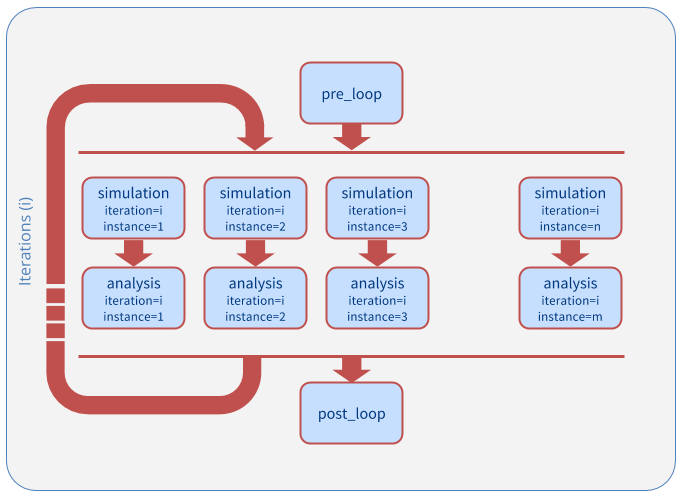
\includegraphics[width=12cm,height=9cm]{sal.png}
  \hbox{\small\itshape Credit: EnsembleMD toolkit architecture document \cite{site1}}
  \caption{Simulation Analysis Loop Pattern}
  \label{fig:sal}
\end{figure}

\section{EnsembleMD Execution Flow}
This section focuses on the flow of application using EnsembleMD toolkit. Figure \ref{fig:modulesofenmd} shows the execution flow of the applications using EnsembleMD tool. At the start of execution, \texttt{radical.entk.Sin
-gleClusterEnvironment} is invoked that calls \texttt{radical.entk.Engine}. Engine module coordinates the patterns and kernel plugins. Engine invokes the loading of all the available patterns, namely, \texttt{radical.entk.pipeline},  \texttt{radical.ensemblemd.exec\_plugins.simulation\_analysis\_loop},  \texttt{radic
-al.ensemblemd.exec\_plugins.replica\_exchange} and \texttt{radical.ensemblemd.exec\_plugins.allp
-airs}. If all of the patterns are loaded successfully, the execution proceeds to the kernel plug-in loading phase; otherwise, it raises exception. This is pattern loading phase takes around 0.0065 seconds.

Next, \texttt{radical.entk.Engine} invokes \texttt{radical.ensemblemd.kernel\_plugins} module and loads all the pre-defined kernels. These loaded kernels are both scientific and miscellaneous. This is kernel plugin loading phase takes around 0.052 seconds. The successful kernel loading process then proceeds to the resource allocation stage.

In the resource allocation stage, control is transferred back to \texttt{radical.entk.SingleClusterEnvi
-ronment} module which is responsible for securing resources on the target machine as requested by the application. On a successful allocation of resource, all the required files are transferred to the target machine, but an exception is raised if the allocation fails and the application exits the execution. Next, the pattern and kernel plugins requested by the application are verified. The next stage is the execution of application on the target machine. After successful execution, EnsembleMD prepares for the de-allocation of the resources. This step is necessary in order to free the reserved resources on the target machine. If the de-allocation process is successful, EnsembleMD exits with a success command and downloads all of the results and outputs, but raises exception if there is any error in any stage of the execution process.

\begin{figure}
  \centering
  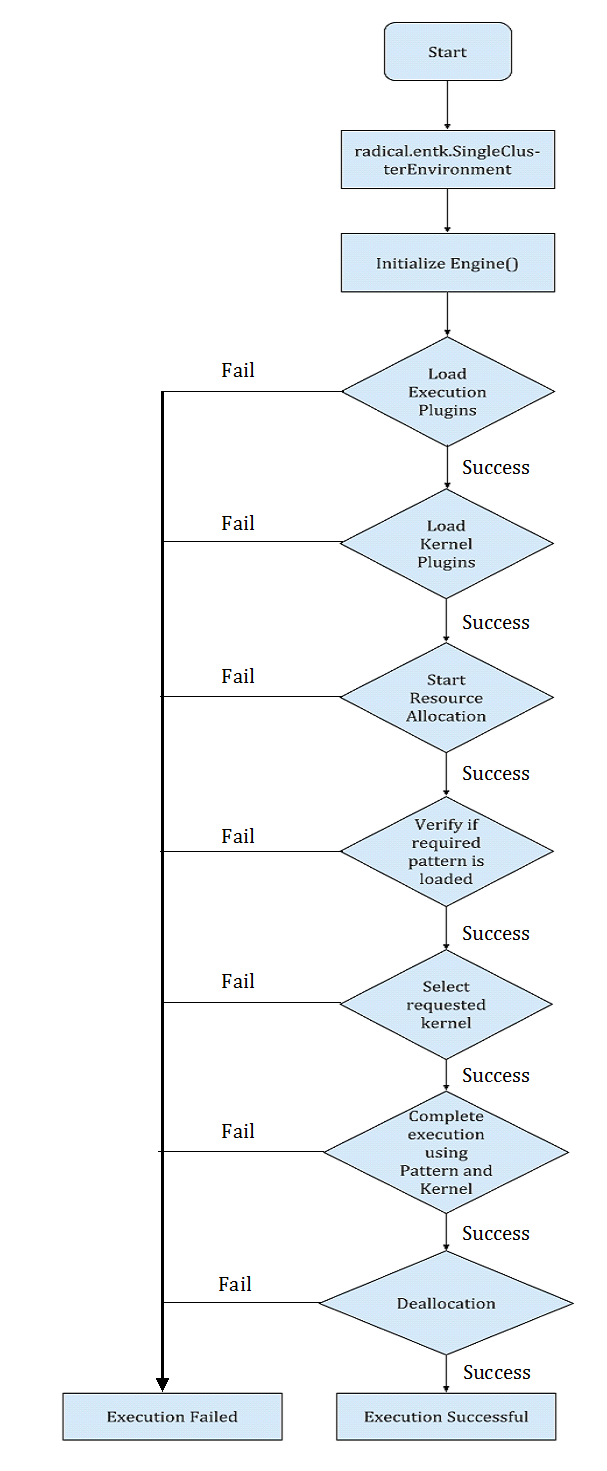
\includegraphics[width=9cm,height=23cm]{ex_flow.png}
  \caption{Sequence of module loading in EnsembleMD toolkit}
  \label{fig:modulesofenmd}
\end{figure}

\begin{landscape}
\begin{figure}
  \centering
  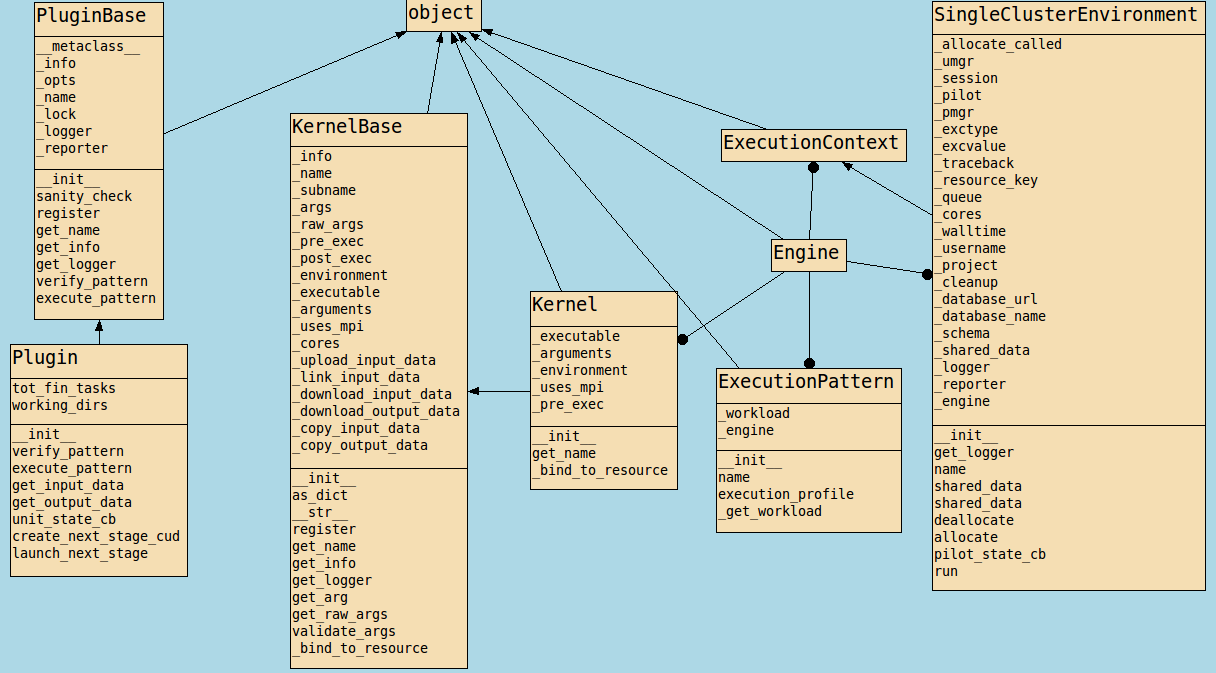
\includegraphics[width=23cm,height=14cm]{complete1.png}
  \caption{UML Diagram of EnsembleMD toolkit}
  \label{fig:umlcomplete}
\end{figure}
\end{landscape}

\begin{figure}[h]
  \centering
  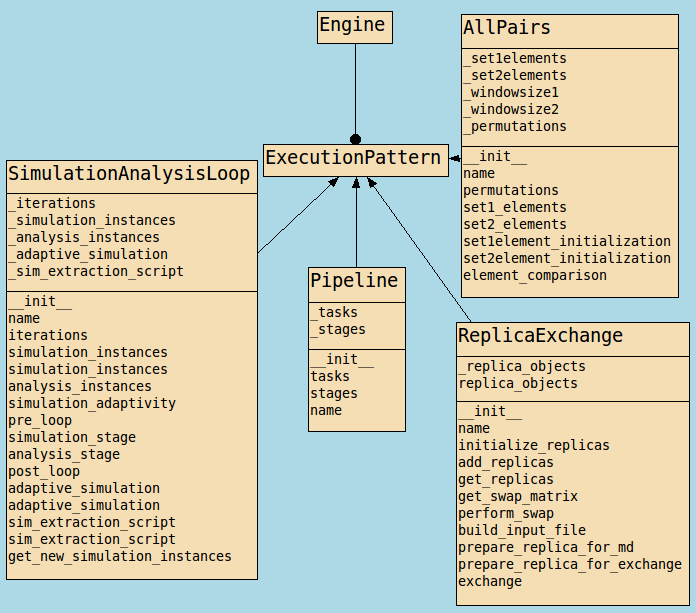
\includegraphics[width=15cm,height=12cm]{pattern.png}
  \caption{UML Diagram of Pattern in EnsembleMD toolkit}
  \label{fig:umlpattern}
\end{figure}

\begin{figure}[h]
  \centering
  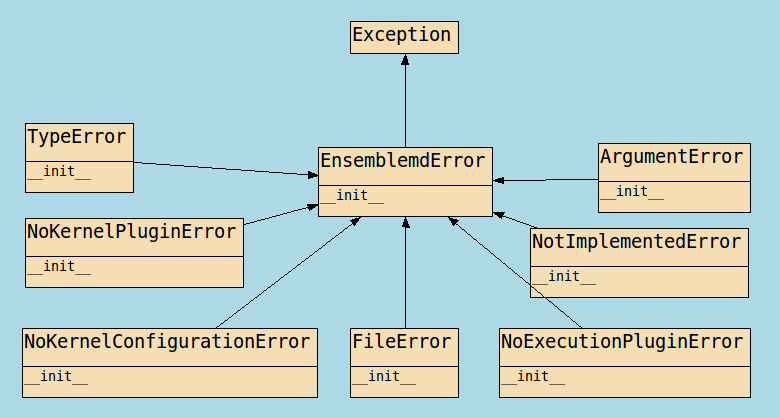
\includegraphics[width=12cm,height=7.5cm]{exception.png}
  \caption{UML Diagram of Exception class in EnsembleMD toolkit}
  \label{fig:umlexception}
\end{figure}


\section{Radical RepEx Framework}
RepEx is a framework for replica exchange molecular dynamics simulations over multiple dimensions. Replica exchange simulation deals with the exchange of thermodynamic information such as temperature, salt concentration or umbrella during molecule interactions, hence supporting 3-dimensional REMD simulations with arbitrary ordering of the available exchange types \cite{ref5}, \cite{site2}.  There are a large number of REMD simulation tools that handles synchronous replica exchanges. In synchronous replica exchange, all the replicas must finish the simulation phase before moving to the next stage, i.e. transition phase \cite{ref5}. RepEx framework not only supports synchronous exchanges, but, it also manages the replicas that do not have global synchronization between the two stages, namely, simulation and exchange phase as shown in figure \ref{fig:repex}. This framework also handles resource allocation for the HPC clusters using underlying Radical Pilot layer.

\begin{figure}

\begin{subfigure}{.5\textwidth}
  \centering
  %\begin{framed}
  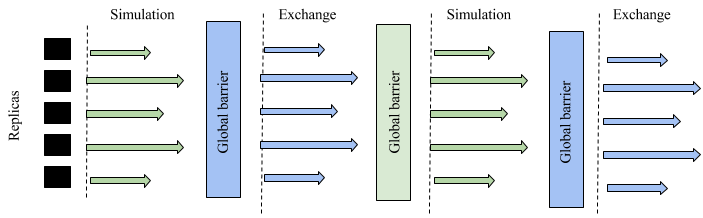
\includegraphics[width=16cm,height=5cm]{Sync.png}
  %\end{framed}
  \caption{Synchronous REMD}
  \label{fig:sync}
\end{subfigure}%
\\
\begin{subfigure}{.5\textwidth}
  \centering
  %\begin{framed}
  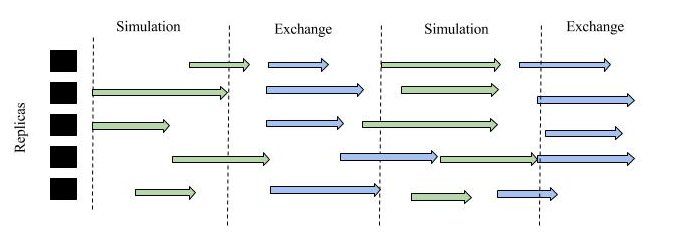
\includegraphics[width=16cm,height=5cm]{async.jpg}
  %\end{framed}
  \caption{Asynchronous REMD}
  \label{fig:async}
\end{subfigure}
\caption{Schematic representation of REMD simulations \cite{ref5}}
\label{fig:repex}
\end{figure}


The main objective for the development of RepEx is to solve the concerns of the scientific community to implement REMD algorithms with a large number of exchanged parameters simultaneously providing a scalable platform with concealed simulation details.


\chapter{Software Testing Framework}

%\section{Importance of Software Testing Framework}
Software testing is the primary way to improve software reliability. Software faults and errors could possibly even cause huge financial damage to users, institutions or corporations. Automatic software testing reduces human efforts by testing the functionality and generating the output reports. This thesis mainly focuses on the development of a testing framework for the projects under Radical Cybertools Group such as EnsembleMD toolkit and RepEx framework. The earlier chapters focused on the EnsembleMD toolkit, its kernels, its patterns and underlying Radical-Pilot framework and concentrated on the importance and requirement of RepEx framework to enhance the domain of REMD simulations. In this chapter, we will discuss the various types of software testing and the importance of each type of testing in the field of computer programming.

\section{Methods of Testing}
%http://www.dcs.gla.ac.uk/~johnson/teaching/safety/powerpoint/15_Testing.pdf
%http://www.angelfire.com/nt2/softwarequality/testestxdin.pdf
%https://www.veracode.com/blog/2013/12/static-testing-vs-dynamic-testing

Edsger W Dijkstra (1930-2002) says,``Testing can prove the presence of errors, but not their absence." In a broader view, testing methods can be divided into two subsections, namely: Static Test and Dynamic Test. These testing methods are also depicted in figure \ref{fig:test_met} for reference.

\begin{figure}
  \centering
  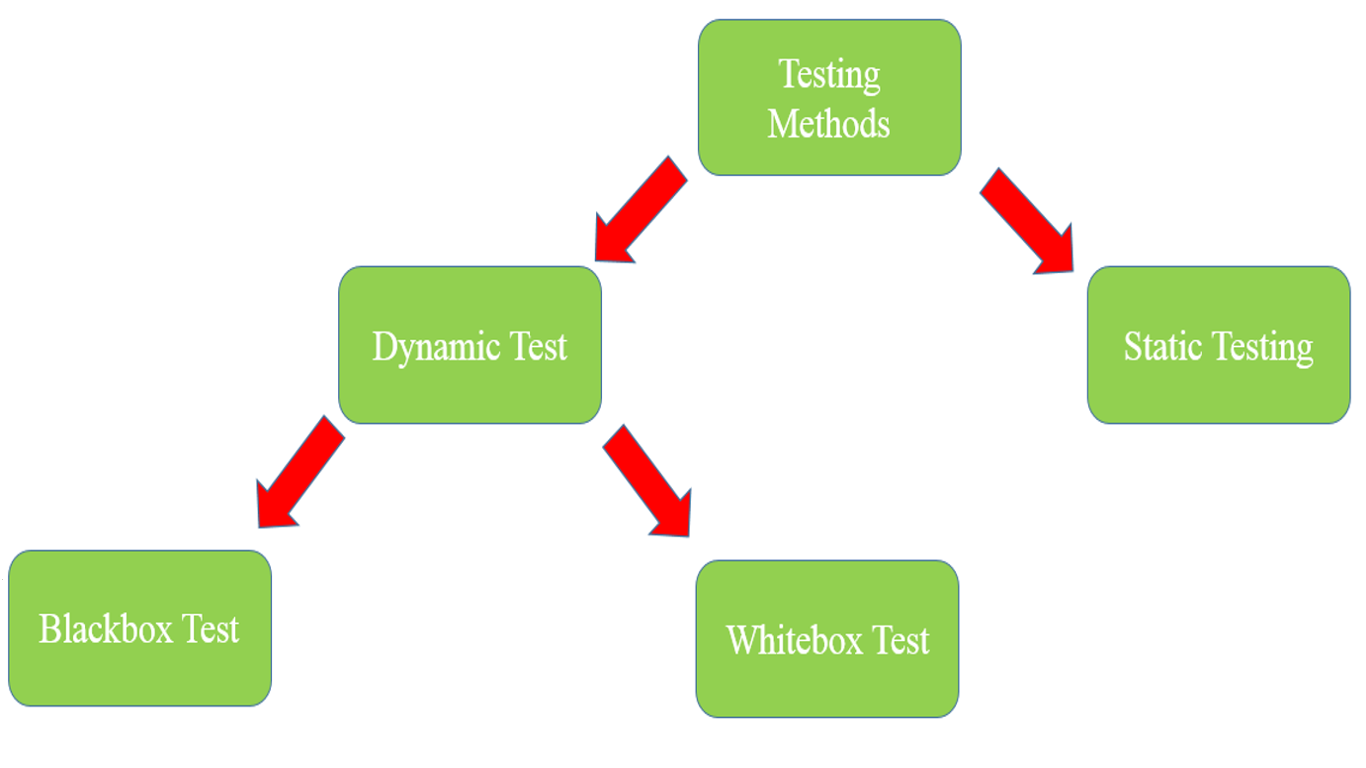
\includegraphics[width=17cm,height=8cm]{test_method.png}
  \caption{Methods of testing}
  \label{fig:test_met}
\end{figure}

\subsection{Static Test}
In software development and testing, Static testing is a technique in which software is tested without executing the code. It gives comprehensive diagnostics for the code. This type of testing mainly has two components \cite{site10}:
\begin{itemize}
%%http://www.tutorialspoint.com/software_testing_dictionary/static_testing.htm
	\item \textbf{Code Review:} It is typically used to find and eliminate the errors in the requirements, code, test cases or associated documents. This includes peer reviews.
	\item \textbf{Static Analysis:} The code written is checked for the proper structure, formatting, syntax correctness and code complexity. It can be tested manually or using some set of tools.
\end{itemize}

\section{Dynamic Test}
This method is used to test the dynamic behavior of the code. It refers to the physical response of the system for various inputs. Unlike the Static test method, Dynamic tests require actual compilation and execution of the code. The actual output for the system for a given input is verified against the expected output. A dynamic test monitors system memory, functional behavior, response time, and overall performance of the system. Dynamic test can be further divided into a Blackbox test and a Whitebox test.

\subsection{Blackbox Testing}
%http://research.ijcaonline.org/volume87/number18/pxc3894024.pdf

Software testing is required to test each module in the code so that maintenance cost can be reduced. Blackbox testing comes into picture when the source code is not available. Blackbox testing completely focuses on the output generated in response to the given input rather than the internal dynamics of the software \cite{ref24}. This focuses on the functionality of the system rather than its implementation and deployment. Figure \ref{fig:bb} shows the block diagram for blackbox testing where the implementation of the system under test is unknown. The only known parameters are the input and the expected output according to the system design document.

\begin{figure}
  \centering
  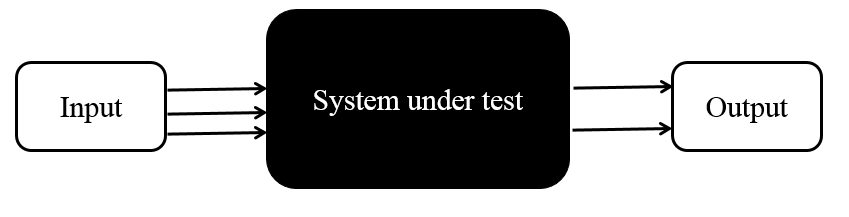
\includegraphics[width=15cm,height=4cm]{bb.png}
  \caption{Block diagram of Blackbox Testing}
  \label{fig:bb}
\end{figure}


\subsection{Whitebox Testing}
Whitebox testing, in contrast to blackbox testing, includes the knowledge of internal code implementation and code flow. In these types of test, all the individual paths, loops in the code structure and all the functions and methods are tested for their logical correctness. Whitebox testing is an important part of the software development cycle of any developing software. A test engineer is required to have a full knowledge of the source code. These tests might be useful in detecting hidden errors, check dead code or other code related bugs \cite{ref25}.

\begin{comment}

\section{Design Aspect for EnsembleMD Toolkit}
We have discussed in detail about the different types of test methods. For this thesis, we will be using Whitebox testing to develop a testing framework which would test the functionality of all the APIs of the EnsembleMD toolkit and RepEx and generate a testing report for the analysis. Radical-Pilot serves as the basic infrastructure for duo. EnsembleMD provides an abstraction over the Radical-Pilot framework exposing the building blocks to the users in form of 'patterns', 'kernels' and 'resource handlers'. This toolkit hides the complexity of resource allocation, job submission, job execution and data transfer from the users, hence, providing easy-to-use plugins to them for developing and executing the molecular dynamics applications. Similarly, RepEx is Replica Exchange MD simulation package providing a scalable solution for multidimensional simulations.

Testing in EnsembleMD toolkit starts right from the resource allocation to the end to end execution of MD applications. Users create an execution context for the target source that would acquire set of resources for the requested period of time. User in the next step selects a execution pattern corresponding to their application and kernel for instantiating specific science tool. These objects are then transferred to the underlying Radical-Pilot layer which then acquires the resources on the remote machine, submit the pilot with compute units and queue them for the execution. 
\end{comment}



\section{Python Testing Tools}
This section focuses on the study of different Python testing tools and selection of the most suitable tool for the testing framework. EnsembleMD toolkit is a Python based framework and hence, Pytest is the most suitable testing tool for the same. The other tools for testing python framework are python unittest/PyUnit, doctest, nose etc which are discussed briefly below.

%http://quintagroup.com/cms/python/python-unit-testing
\subsection{Python unittest/ PyUnit}
Python's unittest framework, developed by Kent Beck and Erich Gamma is based on the XUnit framework. PyUnit supports modularity and is flexible as tests can be organized into test suits with fixtures (setup/teardown). PyUnit supports test fixtures, test cases and a test runner to enable automated testing. The example of unittest is below:

%https://docs.python.org/2/library/unittest.html

%\begin{comment}
\begin{lstlisting}[language=Python]
import unittest
class TestStringMethods(unittest.TestCase):
  def test_upper(self):
      self.assertEqual('foo'.upper(), 'FOO')
if __name__ == '__main__':
    unittest.main()
\end{lstlisting}

\textbf{Output:}

\begin{lstlisting}[language=Python]
Ran 3 tests in 0.000s
OK
\end{lstlisting}
%\end{comment}

\subsection{Doctest}
%https://docs.python.org/2/library/doctest.html
Doctest is simple testing framework that executes a shell script in docstring format in a small function at the bottom of the test file. Doctest enables the test by running examples included in the documentation and verifying the expected results. The test module searches for pieces of text that look like interactive Python sessions, and then executes those sessions to verify that they work exactly as shown in the text. The example of doctest is below:

%\begin{minted}[frame=lines,framesep=15pt]{python}
\begin{lstlisting}[language=Python]
def mul_function(a, b):
>>>mul_function(2,3)
6
return a*b
\end{lstlisting}

\textbf{Output:}

%\begin{minted}[frame=single,framesep=15pt]{python}
\begin{lstlisting}[language=Python]
Trying:
    mul_function(2, 3)
Expecting:
    6
ok
1 tests in 1 items.
1 passed and 0 failed.
Test passed.
\end{lstlisting}


\subsection{Nose}
Nose is an extension of Python unittest to enhance testing. It has several built-in modules which helps to capture error, output, code coverage. Nose, although fully compatible with Python unittest, has a slightly different approach to running tests. Nose lowers the barrier to writing tests and its syntax is less complicated.
The example of Nose test is below:

%\begin{minted}[frame=lines,framesep=15pt]{python}
\begin{lstlisting}[language=Python]
from unnecessary_math import multiply
 def test_numbers_3_4():
    assert multiply(3,4) == 12 
\end{lstlisting}
\textbf{Output:}
%\begin{minted}[frame=single,framesep=15pt]{python}
\begin{lstlisting}[language=Python]
Ran 1 tests in 0.000s
OK
> nosetests -v test_um_nose.py
simple_example.test_um_nose.test_numbers_3_4 ... ok
Ran 2 tests in 0.000s
OK
\end{lstlisting}

\subsection{Pytest}
Py.test is easy and has straightforward asserting with the assert statements. The output description of pytest is better than other test frameworks. It provides a better description whenever the test case fails. Pytest framework has its own runner method to execute the tests with name test\_*.py.

%\begin{minted}[frame=lines,framesep=15pt]{python}
\begin{lstlisting}[language=Python]
def func(x):
    return x + 1
def test_answer():
    assert func(3) == 5
\end{lstlisting}

\textbf{Output:}

%\begin{minted}[frame=single,framesep=15pt]{python}
\begin{lstlisting}[language=Python]
======= test session starts ========
platform linux -- Python 3.4.3, pytest-2.8.7, py-1.4.31, pluggy-0.3.1
rootdir: /home/suvigya/radical.ensemblemd-master, inifile:
collected 1 items
test_sample.py F
======= FAILURES ========
_______ test_answer ________
    def test_answer():
>       assert func(3) == 5
E       assert 4 == 5
E        +  where 4 = func(3)
test_sample.py:5: AssertionError
======= 1 failed in 0.12 seconds ========
\end{lstlisting}

The above results and the output of Pytest is more descriptive and hence, serves as the backbone for our testing framework over the other available test tools. Pytest not only provides better output logging, but also has simpler syntax, is easy to implement and ieasy to integrate with continuous integration tools such as Jenkins or code coverage tools.

\section{EnsembleMD and Repex Test Automation Framework Requirements}
The previous sections discuss the different types of testing methods and tools available and superiority of pytest over other testing tools. This section aims at the basic test structure and requirements of our test infrastructure.

\subsection{High Level Requirements}
The basic requirement of any test framework, especially EnsembleMD and RepEx framework, is described in the table \ref{table1}.

\begin{table}
\begin{center}
\def\arraystretch{2}
\begin{tabular}{|l| p{10cm}|}
\hline
Automatic Test Execution & The primary requirement of the test framework is to execute the test automatically along with error reporting, test analysis and test report generation. \\ 
\hline
Convenience & Framework must be easy and convenient to use by the testers/ developers and must be easy to edit and add more tests. \\ 
\hline
Maintainability & Framework should be easy to maintain and update the test results as soon as any changes have been made in the source code or any changes have been pushed to the repository.\\ 
\hline
\end{tabular}
\end{center}
\caption{Basic testing infrastructure requirements}
\label{table1}
\end{table}

\subsection{Test Framework Capabilities}
The flows chart in figure \ref{fig:flowchart} depicts the capabilities of a test execution framework.
\begin{figure}
  \centering
  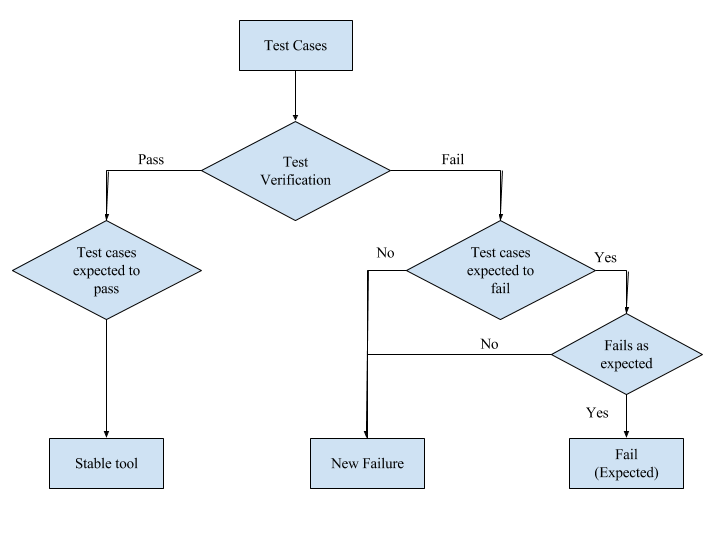
\includegraphics[width=15cm,height=10.5cm]{flowchart.png}
  \caption{Test Execution Flow}
  \label{fig:flowchart}
\end{figure}

\begin{itemize}

\item \textbf{Starting or Stopping tests}\newline
As EnsembleMD toolkit and RepEx are evolving open source projects, where functionalities, APIs and source code is always changing and and modified, it is important for the test infrastructure to start testing the updated source code with any new pushed changes automatically. This ensures that the functionality of the overall system is intact and flawless. The framework should also start executing these tests at some frequent intervals to ensure that even a software upgrade on the remote HPC clusters are properly captured and source code of scientific applications is modified accordingly to make it compatible with the upgrades.

\item \textbf{Test Report Generation}\newline
Test reports generated after each automated testing is very crucial. These test reports are not only important for test engineers, but also significant for the developers. Test reports elucidates developers about the failing modules. These reports provide steps or inputs to reproduce the error which is beneficial at the later stage to re-test the bug-fix provided by the developers. 

\item \textbf{Verifying Test Results}\newline
Verifying the test results is the integral part of test execution. Tests can be verified by comparing the actual output with the predefined expected output.

\item \textbf{Handling Expected Failures}\newline
The essential part of any test execution is to verify and handle the failures. The analysis of the test failures is important to ascertain that the known to fail test cases have failed similarly as expected or new defects have appeared. A test framework is expected to distinguish between the expected test failures and the new test failures on the basis of the expected output for a test failure. Hence, when a test case fails, the expected failed output is compared against the actual outcome. If the outcome matches an expected failure is detected, otherwise a new failure, defect or bug is detected. 

\end{itemize}

The complete design of testing framework and the error detection is divided into 3 levels:

\begin{itemize}
\item \textbf{Development level testing:} This is the basic API level testing of the EnsembleMD tool kit and RepEx framework.
\item \textbf{Deployment level testing:} This includes testing for the errors that occurs during loading the environment, modules or the errors that arise during the transfer of scientific tool dependent input files on to remote machines. 
\item \textbf{Run-time testing:} This level of testing framework deals with the execution failure of scientific tools due to various reasons which is discussed in further chapters. 
\end{itemize}

In our testing framework, Development level testing includes unit testing of all the independent functionalities of EnsembleMD tool kit and RepEx framework which is discussed in the next chapter. We have designed Simple Application Testing Lite (SATLite), an independent framework for testing deployment and run-time level errors and faults. SATLite detects the errors using console logs of the supercomputer.


%Chapter 5
\chapter{Development-level Testing}

\section{Introduction}
The previous chapter briefly discussed the various testing tools and design features required for developing a test infrastructure for the EnsembleMD toolkit and RepEx. This chapter focuses mainly on the API level testing of all the patterns APIs, kernel APIs and execution handler APIs of EnsembleMD toolkit. The testing infrastructure is divided into Unit Testing, End to End Testing and Exception testing which are described in detail in this chapter.

\section{Unit Testing}
Unit tests are written and executed by the developers to ensure that the output of the code meets the design of the software. In the field of software programming, unit testing is a method to test the individual modules or units of the code to verify its proper functioning. 

Pytest was chosen because of the following features:
\begin{itemize}
\item It collects all the test files automatically as it looks for file names starting with test\_*.py.
\item It has simple asserts and highly customizable debugging logs and output.
\end{itemize}

\subsection{Unit test for EnsembleMD toolkit}
All the different APIs of all the patterns forms the building block of EnsembleMD toolkit. Different APIs of a pattern can execute as an individual module with or without data dependency from previous stages. In general, Unit Testing for EnsembleMD toolkit pattern is divided into three modules as shown in figure \ref{fig:ut}, namely: 

\begin{itemize}
\item \textbf{Basic Api Test module:} It tests the basic APIs of the patterns viz import module test, name of the pattern, check the variables etc.
\item \textbf{Not Implemented Error test module:} The important feature of EnsembleMD toolkit is to generate error and throw exception when the pattern API or function is not defined or given any functionality. In this case, toolkit raises \texttt{NotImplementedError} error. In this module, we test the function without definition and the exceptions raised. 
\item \textbf{Implemented API module:} In this module, we define the APIs of the pattern and provide them functionality. These functions are given required inputs and are tested for the expected output. This tests all of the APIs which generated \texttt{NotImplementedError} by defining them and executing them with specific input data or files.
\end{itemize}

\begin{figure}
  \centering
  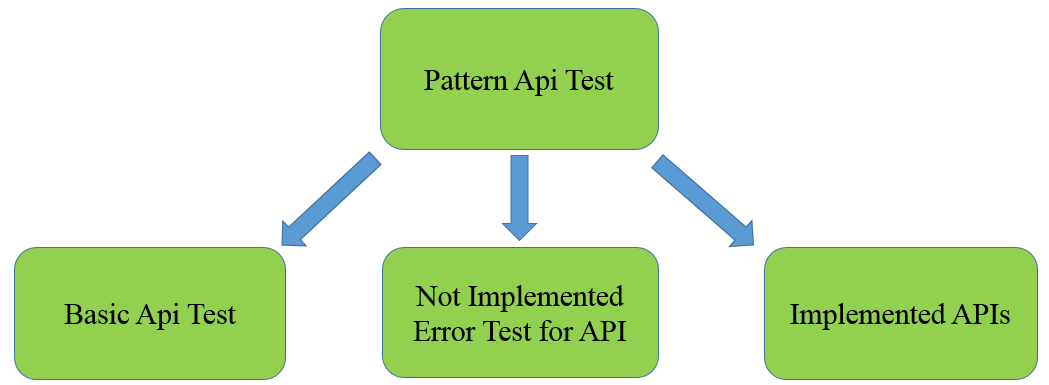
\includegraphics[width=17cm,height=6cm]{ut.png}
  \caption{Unit Testing modules}
  \label{fig:ut}
\end{figure}

Table \ref{enmdapitable} shows all the APIs of the patterns which were included in unit testing.

\begin{table}
\begin{center}
\begin{tabular}{|p{2cm}|p{3cm}|p{5cm}|p{5cm}|}
\hline
\rule{0pt}{15pt} \textbf{Pattern} & \textbf{Basic API} & \textbf{Not Implemented API} & \textbf{Implemented API} \\[2ex]
\hline
Pipeline & 
	\begin{itemize}
	\item import pipeline module
	\item name
	\item instances
	\item steps
	\end{itemize}
	& 
	\begin{itemize}
		\item step\_n
	\end{itemize}
	& 
	\begin{itemize}
		\item step\_n
	\end{itemize}
	\\
\hline
AllPairs &
	\begin{itemize}
	\item import
	\item name
	\item permutations
	\item set1\_elements
	\item set2\_elements
	\end{itemize}
	&
	\begin{itemize}
	\item set1element\_initialization
	\item set2element\_initialization
	\item element\_comparison 
	\end{itemize}
	&
	\begin{itemize}
	\item set1element\_initialization
	\item set2element\_initialization
	\item element\_comparison 
	\end{itemize}
	\\
\hline
Replica Exchange &
	\begin{itemize}
	\item import
	\item name
	\item add\_replica/
	get\_replica
	\end{itemize}
	&
	\begin{itemize}
	\item initialize\_replica()
	\item build\_input\_file
	\item get\_swap\_matrix
	\item perform\_swap
	\item prepare\_replica
	\_for\_md
	\item prepare\_replica
	\_for\_exchange
	\item exchange 
	\end{itemize}
	&
	\begin{itemize}
	\item initialize\_replica()
	\item build\_input\_file
	\item get\_swap\_matrix
	\item perform\_swap
	\item prepare\_replica
	\_for\_md
	\item prepare\_replica
	\_for\_exchange
	\item exchange 
	\end{itemize}
\\
\hline
Simulation Analysis Loop &
	\begin{itemize}
	\item import
	\item name
	\item iterations
	\item simulation
	\_instances
	\item analysis
	\_instances
	\item simulation
	\_adaptivity
	\end{itemize}
	&
	\begin{itemize}
	\item pre\_loop()
	\item simulation\_step()
	\item analysis\_step()
	\item post\_loop() 
	\end{itemize}
	&
	\begin{itemize}
	\item pre\_loop()
	\item simulation\_step()
	\item analysis\_step()
	\item post\_loop() 
	\end{itemize}
\\
\hline
\end{tabular}
\end{center}
\caption{Pattern APIs for Unit Testing in EnsembleMD toolkit}
\label{enmdapitable}
\end{table}



\begin{comment}

\section{Integration Testing}
Integration Testing is a quality assurance process in which a group of modules or components are tested combinly to generate an output. This type of testing takes the unit tested input modules, groups them in larger group and applies test defined in the test plan. In EnsembleMD toolkit, we combined pattern APIs with the resource allocation handler, hence tested proper resource allocation, deallocation and running.  Figure \ref{fig:int} depicts the flow of Integration testing. In integration, we mainly tested the APIs of resource handler which allocates and deallocates the resources combined with pattern APIs.\newline
This is the pseudo code for resource handler. 
\begin{lstlisting}[language=Python]
#Pseudo code 
Define Pipeline API
Create resource handler with resource configuration
allocate()
Call pattern
run() with pattern
deallocate()
\end{lstlisting}

\newline Test resource allocation
\begin{lstlisting}[language=Python]
    #Test allocate()
    def test_allocate(self,enmd_setup):
        ret_allocate,ret_deallocate = enmd_setup
        assert (ret_allocate == True)
\end{lstlisting}

\newline Test resource deallocation
\begin{lstlisting}[language=Python]
    #Test deallocate()
    def test_deallocate(self,enmd_setup):
        ret_allocate,ret_deallocate = enmd_setup
        assert (ret_deallocate == True)
\end{lstlisting}

\newline Test running kernel and pattern on remote machine
\begin{lstlisting}[language=Python]
    #Test run()
    def test_run(self,enmd_setup_run):
        ret_allocate,ret_run,ret_deallocate = enmd_setup_run
        assert ret_run == True
\end{lstlisting}

\begin{figure}
  \centering
  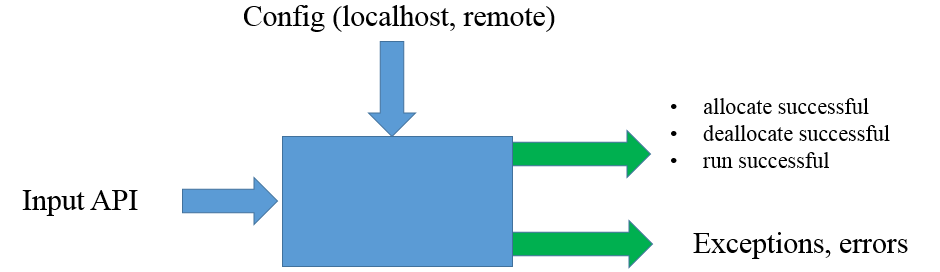
\includegraphics[width=17cm,height=5cm]{int.png}
  \caption{Integration Testing Flow}
  \label{fig:int}
\end{figure}
\end{comment}


\subsection{Unit test for RepEx toolkit}
Unlike EnsembleMD toolkit, RepEx framework is a modifiable and scalable REMD simulation package that supports Amber and NAMD as molecular dynamics application kernels. The most important stage in any replica exchange simulation is the initialization of the replicas and the number of replicas in each dimensional group. Errors propagate to the next stage if the initialization of replicas is faulty and hence providing erroneous results. These errors in the final output might cause severe damages if the results are used in the development of drugs [1].

As discussed earlier, RepEx supports one dimensional simulations with temperature exchange, umbrella sampling and salt concentration. These one dimensional simulations can be combined to perform multidimensional exchange simulations. The test cases for the RepEx extensively focuses on the replica initialization part. Table \ref{repexapitable} shows the important test cases scenarios of RepEx. These test cases are executed for all the dimensions for all the possible combinations; moreover, these test cases also checks for errors in synchronous and asynchronous modes of execution.

\begin{table}
\begin{center}
\def\arraystretch{2}
\begin{tabular}{|p{4cm}|p{5cm}|p{6cm}|}
\hline
\rule{0pt}{15pt} \textbf{Test Cases} & \textbf{Usage} & \textbf{If test fails} \\[2ex]
\hline
test\_initialize\_replica\_id &
Tests the IDs of all the replicas that are initialized. &
Wrong replica IDs would lead to improper exchange and tracking of replicas at the later stages.
\\
\hline
test\_total\_group &
Tests the total number of groups generated. &
Incorrect group number would lead to improper exchanges.
\\
\hline
test\_group\_d1 &
Tests for the proper number of replicas in D1 dimension. &
Incorrect numbers would lead to error propagation to next stages and improper exchanges.
\\
\hline
test\_group\_d2 &
Tests for the proper number of replicas in D2 dimension. &
Incorrect numbers would lead to error propagation to next stages and improper exchanges.
\\
test\_group\_d3 &
Tests for the proper number of replicas in D3 dimension. &
Incorrect numbers would lead to error propagation to next stages and improper exchanges.
\\
\hline
\end{tabular}
\end{center}
\caption{Test cases for Unit Testing in RepEx}
\label{repexapitable}
\end{table}


\section{End-to-End Testing}
End-to-end testing tests the complete functionality of all the patterns starting from the selecting pattern, defining kernel and allocating resource. Each pattern is tested with a specific input and compared with the expected output. These tests ensures the proper functioning and behavior satisfaction of the complete toolkit. The End-to-end testing on different supercomputers helps in establishing reliability of the toolkit. 

End-to-end testing includes testing all the miscellaneous kernels along with the scientific tool kernels (Amber, CoCo, Gromacs and LSDMap). These tests are executed on both localhost and Stampede supercomputer.

\begin{comment}
Discussed below is the code snippet for End-to-end test for pipeline pattern.

\begin{itemize}
\item Creating the Execution Context
\begin{lstlisting}[language=Python]
cluster = SingleClusterEnvironment(
                  resource=resource,
                  cores=1,
                  walltime=15,
                  username=config[resource]['username'],
                  project=config[resource]['project'],
                  access_schema = config[resource]['schema'],
                  queue = config[resource]['queue'],
                  database_url='mongodb://suvigya:temp123@
ds051585.mongolab.com:51585/rutgers_thesis'         )
cluster.allocate()
\end{lstlisting}

\item Defining the Pattern details
\begin{lstlisting}[language=Python]
randomsa = RandomSA(maxiterations=1, simulation_instances=1, 
		     analysis_instances=1)
cluster.run(randomsa)
\end{lstlisting}

\item Creating Simulation-Analysis Class
\begin{lstlisting}[language=Python]
class RandomSA(SimulationAnalysisLoop):
def __init__(self, maxiterations, 
			simulation_instances=1, 
			analysis_instances=1):
	SimulationAnalysisLoop.__init__(self, 
			maxiterations, 
			simulation_instances, 
			analysis_instances
		)
\end{lstlisting}

\item Defining the ’pre-loop’
\begin{lstlisting}[language=Python]
def pre_loop(self):
    k = Kernel(name="misc.mkfile")
    k.arguments = ["--size=1000", "--filename=reference.dat"]
    k.upload_input_data = ['levenshtein.py']
    return k
\end{lstlisting}

\item Defining Simulation loop
\begin{lstlisting}[language=Python]
def simulation_step(self, iteration, instance):
    k = Kernel(name="misc.mkfile")
    k.arguments = ["--size=1000", "--filename=simulation-{0}-{1}.
dat".format(iteration, instance)]
    return k
\end{lstlisting}

\item Defining Analysis loop
\begin{lstlisting}[language=Python]
def analysis_step(self, iteration, instance):
    input_filename  = "simulation-{0}-{1}.dat".
format(iteration, instance)
    output_filename = "analysis-{0}-{1}.dat > /home/suvigya/Blackbox
/analysis-{0}-{1}.dat".format(iteration, instance)
    k = Kernel(name="misc.levenshtein")
    k.link_input_data      = ["$PRE_LOOP/reference.dat", 
"$SIMULATION_ITERATION_{1}_INSTANCE_{2}/{0}".
format(input_filename,iteration,instance),"$PRE_LOOP/levenshtein.py"]
    k.arguments = ["--inputfile1=reference.dat",
                   "--inputfile2={0}".format(input_filename),
                   "--outputfile={0}".format(output_filename)]
    k.download_output_data = output_filename
    return k
\end{lstlisting}

\item Test Case for End to end checking
\begin{lstlisting}[language=Python]
assert os.path.isfile("./analysis-1-1.dat")
os.remove("./analysis-1-1.dat")
\end{lstlisting}
\end{itemize}
\newline This checks if the analysis-1-1.dat is generated in the Simulation Analysis loop execution as expected. The test case fails if the file is not generated indication some exception or error occurred during execution.
\end{comment}


\section{Exception Testing}
The EnsembleMD toolkit and RepEx provides a well detailed logging for the errors and exceptions. It generates very specific exceptions which helps in debugging the failure at any step. We provide wrong or improper inputs to check if these exceptions are raised. Table \ref{exception} shows important exceptions provided by the two Radical toolkits.

\begin{table}
\begin{center}
\def\arraystretch{2}
\begin{tabular}{|p{4cm}|p{5cm}|p{6cm}|}
\hline
\rule{0pt}{15pt} \textbf{Test Case} & \textbf{Exception Raised} & \textbf{Remarks} \\[2ex]
\hline
test\_TypeError &
radical.ensemblemd.exceptions.
TypeError &
TypeError is thrown if a parameter of a wrong type is passed to a method or function.
\\
\hline
test\_FileError &
radical.ensemblemd.exceptions.
FileError &
FileError is thrown if something goes wrong related to file operations, i.e., if a file does not exist or cannot be copied.
\\
\hline
test\_ArgumentError &
radical.ensemblemd.exceptions.
ArgumentError &
This exception is thrown if a wrong set of arguments are passed to a kernel.
\\
\hline
test\_NoKernelPluginError &
radical.ensemblemd.exceptions.
NoKernelPluginError &
This exception is thrown if no kernel plug-in could be found for a given kernel name.
\\
\hline
test\_NoKernelConfigur-
ationError &
radical.ensemblemd.exceptions.
NoKernelConfigurationError &
This exception is thrown if no kernel configuration could be found for the provided resource key.
\\
\hline
\end{tabular}
\end{center}
\caption{Test cases for raising exceptions}
\label{exception}
\end{table}

\begin{comment}
\section{Cognitive Study of EnsembleMD}
Chapter \ref{chap:background} profoundly discusses about the features and design of the various components of EnsembleMD toolkit. In this section, we performed a cognitive analysis of different modules of the former toolkit. A detailed analysis of the modules was conducted to understand the current system and the time each modules require for execution. This study will be helpful to the developers in minimizing the time taken by the EnsembleMD overheads. Logarithmic graph in figure \ref{fig:time_graph} shows the sequence of loading of various modules at run-time execution of examples using EnsembleMD toolkit on localhost. Graph \ref{fig:time_graph} shows that loading and initialization time for pattern and kernel plug-ins are 0.0065 seconds and 0.0052 seconds respectively but the time taken by the execution context API for resource allocation and deallocation is much higher, i.e. 26.53 seconds. Execution context has 3 APIs, namely, allocate(), run() and deallocate(). Graph \ref{fig:ex_context_time} shows the time taken for allocation and de-allocation of the resource. We have only focused on allocation and de-allocation since these APIs are specific to the EnsembleMD tool, but the time taken to execute run() API depends on various factors such as type of application, job scheduling and pending time on target machine, etc. Allocation of resources takes 15.71 seconds on average while de-allocation takes around 10.81 seconds.



\begin{figure}
  \centering
  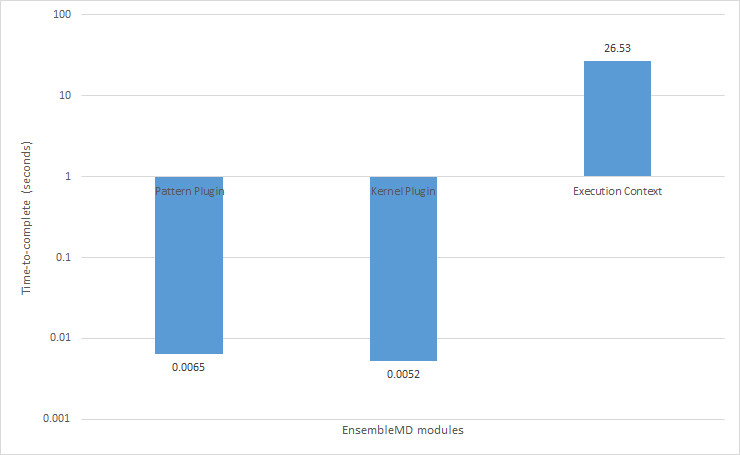
\includegraphics[width=12cm,height=7cm]{mod_time.png}
  \caption{Time to complete module loading (Semi-Log Scale)}
  \label{fig:time_graph}
\end{figure}

\begin{figure}
  \centering
  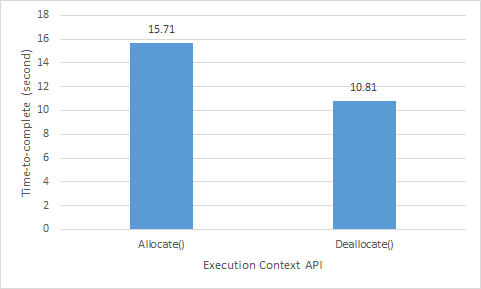
\includegraphics[width=12cm,height=7cm]{ex_context_time.png}
  \caption{Time to complete Execution Context API}
  \label{fig:ex_context_time}
\end{figure}

\end{comment}


\chapter{Deployment and Run-time Testing}

Deployment testing is the next level of testing that captures the exceptions, faults and errors that might occur during the deployment of input files on HPC cluster or loading the scientific tool specific modules and environment on to the supercomputer. Run-time testing focuses on the exceptions that occur due to system failure or segmentation faults. In this thesis, we have carefully designed a framework that checks for the above discussed levels of testing. Simple Application Testing Lite (SATLite) is primarily developed with an objective to test errors and exceptions which occurs during the execution of scientific tools (Amber, Coco, Gromacs, LSDMap etc) on remote supercomputers. 

According to \cite{ref6}, 1.53\% of the total applications on Blue Waters supercomputer failed because of the system problems. Such system failures have a great impact on the computing resources and financial budgeting. The majority of testing tools that have been developed focuses on testing the failures due to system faults, both software and hardware. LogDiver, a tool primarily developed by Martino et al. \cite{ref6} analyzes the system level faults. Failures in HPC clusters have become more prominent with the enhancement in the number of components. The exponential increase in the failures calls for immediate actions to minimize the effect of failed applications on the high computing resources. In this chapter, we focus on application side failure detection. 

\subsection{Basic Definitions}
A few terms related to the development of testing frameworks are discussed below:
\begin{itemize}
\item \textbf{Modules:} Basic environment for the default compilers, tools, and libraries. Users requiring 3rd party libraries or tools can tailor their  environment with the applications and tools they need. Module and environment can be used interchangeably.

\item \textbf{Files:} User's input files specific for the scientific tool

\item \textbf{Supercomputer:} These are the high performance computing resources that are used for the execution of applications. HPC cluster, remote machines and supercomputers can be used interchangeably.

\item \textbf{Scientific tools:} These are the MD simulation tools such as Amber, CoCo, Gromacs and LSDMap. These tools are developed by ExTASY group [10].
\end{itemize}

SATLite tool can help the developers of the scientific community, especially the Molecular Dynamics community to investigate the errors and issues that may be generated due to their software bugs or the remote system changes and upgrade. This enables them to test the changes which have been made in their tools before releasing it for their users. The errors and exceptions might occur due to the following occurrences:

\begin{itemize}
\item Improper or obsolete module loading.
\item Improper input arguments or input files.
\item System failure or segmentation fault.
\item Failure as the execution did not complete in expected range of time.
\end{itemize}

\section{SATLite System Design}

Figure \ref{fig:satdesign} shows the block diagram of the system. SATLite tool performs the test in two steps, i.e. Module Test and Execution Test. In figure \ref{fig:satdesign}, user attributes field depicts the APIs exposed to the users. These APIs are explained in the later sections. Resource configuration file and scientific tool specific defaults modules file serves as the input to this testing tool. 

\begin{figure}
  \centering
  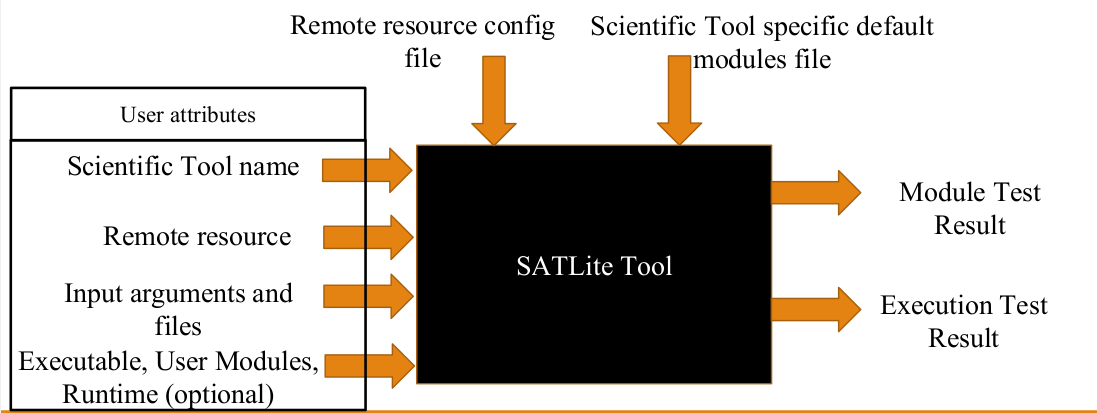
\includegraphics[width=16cm,height=6cm]{satlite_design.png}
  \caption{SATLite System Design}
  \label{fig:satdesign}
\end{figure}

\section{System Architecture}
As a part of SATLite design and development, the primary focus is to report the exceptions and errors occurred due to inadmissible loading of the environment or improper input files on the supercomputer. The continuous development in the scientific tools and changes in their source code raised a requirement to develop a tool that can report any errors relating to its execution on the remote supercomputers.

\begin{figure}
  \centering
  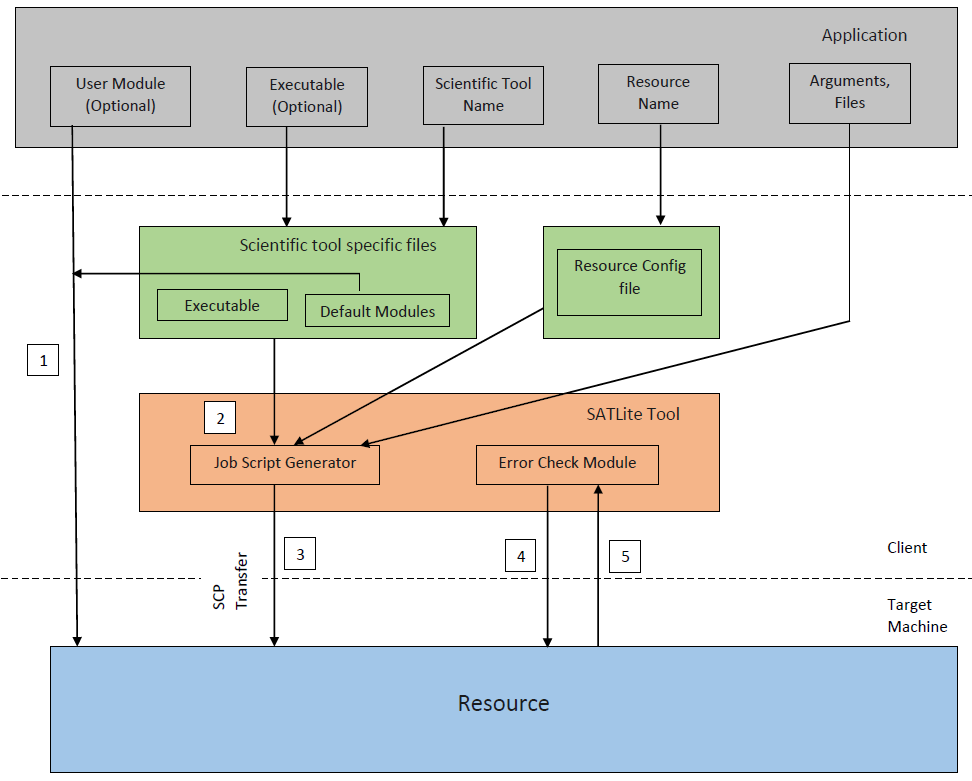
\includegraphics[width=14cm,height=12cm]{satlite.png}
  \caption{SATLite tool architecture}
  \label{fig:satarch}
\end{figure}

SATLite tool provides a set of explicit APIs to the users to test their own scientific tool or application. It has been currently tested for Amber, CoCo, Gromacs and LSDMap. The environment loading, file transfer, job scheduler script generation and its execution is hidden from the users, hence, they can solely focus on the development of scientific tools rather than concentrating on debugging the errors and exceptions.

\subsection{Control Flow}
The control flow for two stages of the SATLite as shown by specific numbers in figure \ref{fig:satarch} are discussed below.

\subsubsection{Module Test}
\textbf{\{1\}} Load user provided or defaults modules on the supercomputer and wait for the console logs. If the user does not explicitly provides any input modules, then the default modules from the scientific tool specific file are used. These console logs are examined to check for the errors during the environment loading stage. If any error event occurs at this stage, the logs are written to the module\_error log file explaining the possible reason for failure.

\subsubsection{Execution Test}
\textbf{\{2\}} Generate job scheduler script using scientific tool executable, modules for a specific remote machine using remote machine configuration file. \newline
\textbf{\{3\}} All the input files along with the scheduler script is transferred to the remote machine using secure copy protocol (SCP). The errors and exceptions are detected, if any, during the file transfer stage. If all the files are transferred successfully, the job is submitted to the computing resource queue where the tools waits for execution to complete.\newline
\textbf{\{4\}} Output files and error files are generated and these log files are examined to detect any failure during execution.\newline
\textbf{\{5\}} At the last stage, errors are reported back to the users. Also, all the output files and error files are transferred back to the local machine. 

\section{System Log Collection and Processing}
We begin by examining the details of the cluster, event methodology and then its processing.

\subsection{About the Cluster: Stampede}
We have currently tested SATLite on the Stampede supercomputer from TACC. Stampede is one of the most powerful supercomputers which went into production in 2013. In 2012, a pre-production configuration of Stampede used 1875 nodes which were then expanded to 6400 node with a total memory of 205 TB. The project was built in partnership with Intel, Mellnox and Dell. Table \ref{stampedespec} shows the technical details of Stampede.

\begin{table}
\begin{center}
\def\arraystretch{1.5}
\begin{tabular}{|p{3cm}|p{10cm}|}
\hline
\rule{0pt}{15pt} \textbf{Resource} & \textbf{Specification} \\[2ex]
\hline
\# of Nodes & 6400
\\
\hline
Processors & Xeon E5-2680 8-core processors
\\
\hline
Co-processor & Xeon Phi coprocessor
\\
\hline
Memory & 32 GB RAM, 205 TB total memory
\\
\hline
GPU & Nvidia Kepler K20 GPUs
\\
\hline
Operations & 9.6 quadrillion floating point operations per second
\\
\hline
\end{tabular}
\end{center}
\caption{Stampede system specifications}
\label{stampedespec}
\end{table}

\subsection{Event Logs and Processing}
Supercomputers such as Stampede logs all the events that occurs during the complete execution of the application. System logs serves as the repository of the event data. Console logs provide the real-time job status. We have utilized these console logs to detect the deployment time and run-time errors. In the deployment stage, it is highly likely that the modules required to run a scientific tool and workflow are erroneous or have become obsolete. The events generated on the console logs are analyzed to provide the explanation of the error.

In the run-time stage, we have used console logs to extract job id, job status, execution time etc. When a batch job exits \cite{ref6}, Stampede generates an exit code which shows the completion status. A successful and exception-free execution returns ExitCode 0 as return code, otherwise an integer greater than 0 depicting different types of errors and exceptions. It is also possible that a job can finish successfully even if the application has terminated abnormally. To address this case, we have used the actual execution time to complete and checked if it lies in the expected range of completion time.

\section{SATLite Tool Components}
The components exposed to the users are discussed below. These components are the parameters that are required to be set using set\_attribute().

\subsection{Scientific Tool Name}
This is the field where the user has to provide the scientific tool name (currently supported scientific tool name are Amber, CoCo, Gromacs and LSDMap) that has to be tested. For example,

\begin{lstlisting}[language=Python,linewidth=3.7cm]
  name = amber
\end{lstlisting}

\subsection{Resource Name}
The input to this field is the name of the supercomputer or any target machine where the execution of the scientific tool has to be checked. This currently supports SLURM job scheduler. For example,

\begin{lstlisting}[language=Python,linewidth=5.7cm]
 resource = xsede.stampede
\end{lstlisting}


\subsection{Arguments}
The list of input files specific to the scientific tools along with the arguments are provided in a specific format as shown in the example below.

\begin{lstlisting}[language=Python,linewidth=13cm]
 arguments = ['argument1=input_file1','argument2=input_file2]
\end{lstlisting}

\subsection{Exe}
This is an optional field where the users can provide their executable which then overrides the default executable.

\subsection{User Modules}
This is an optional field where user can explictly provide the required environments. The in-built modules specific to scientific tools (Amber, CoCO, Gromacs and LSDMap) are used if no user modules are provided.

\subsection{Run-time}
Users can provide an estimate range for run time to check for additional execution failures if no exit code or error is found. The actual run time of the execution should lie in the runtime range provided by the user. It is provided in the following format:

\begin{lstlisting}[language=Python,linewidth=12cm]
 runtime = [``min_time(hh:mm:ss)",``max_time(hh:mm:ss)"]
\end{lstlisting}

\begin{table}
\begin{center}
\def\arraystretch{1.5}
\begin{tabular}{|p{4cm}|p{5cm}|p{6cm}|}
\hline
\rule{0pt}{15pt} \textbf{Function Name} & \textbf{Arguments} & \textbf{Description} \\[2ex]
\hline
set\_attribute &
	\begin{itemize}
	\item name,
	\item resource,
	\item arguments,
	\item exe (optional),
	\item modules (optional),
	\item runtime (optional)
	\end{itemize} &
Sets all the required attributes for execution
\\
\hline
run &
void &
Executes test
\\
\hline
\end{tabular}
\end{center}
\caption{Exposed SATLite tool APIs}
\label{satapi}
\end{table}

\section{Execution}
There are two ways for the users to execute the SATLite, namely:
\begin{itemize}
\item Command Line Tool
\item Use the exposed APIs in the code.
\end{itemize}

\subsection{Command Line Tool}
To run SATLite using command line tool, users are required to provide the scientific tool name, target remote machine and arguments file or a file with the list of input files that are required for the execution of the scientific tool. Users can also provide optional executable name and module file explicitly. They can also provide optional execution runtime range. It is recommended to provide a runtime range so as to enhance the failure reporting. The resulting invocation of SATLite should be:

\begin{lstlisting}[language=Python, linewidth=16cm]
 python satlite_exe.py --name <scientific_tool_name> --resource 
 <target_resource_name> --arguments <argument_file>  --exe <Optional
 _executable>  --modules <optional_module_file> --runtime <Optional
 _runtime_range>
\end{lstlisting}

Where,
\begin{lstlisting}[language=Python, linewidth=16cm]
scientific_tool_name = Scientific Tools (Amber, CoCo, Gromacs, LSDMap)
target_resource_name = Remote Supercomputer Name (Currently tested on 
                       Stampede)
argument_file        = File of list of input files with arguments
Optional_executable  = Executable
optional_module_file = File with list of modules
Optional_runtime_range= Runtime range in format [min_time, max_time] in
                        hh:mm:ss
\end{lstlisting}

\subsection{Use the exposed APIs in the code}
This section provides a guide for using the APIs exposed to the users. The below mentioned example executes Amber on Stampede.

\begin{lstlisting}[language=Python, linewidth=16cm]
"""
Sample Code
"""
from satlite import SATLite

if __name__ == "__main__":
     test = SATLite()
     test.set_attribute(name = 'amber',
                       resource = 'xsede.stampede',
                       # amber
                       arguments = ['-O',
                              '-i=/home/suvigya/inp/min.in',
                              '-p=/home/suvigya/inp/penta.top',
                              '-c=/home/suvigya/inp/penta.crd',
                              '-inf=/home/suvigya/inp/min.inf',
                              '-r=/home/suvigya/inp/md.crd',
                              '-ref=/home/suvigya/inp/min.crd'],
                      #Executable optional
                      exe = sander
                      #amber modules optional
                      modules = ["module load TACC",
                            "module load intel/13.0.2.146",
                            "module load python/2.7.9",
                            "module load netcdf/4.3.2",
                            "module load hdf5/1.8.13"]
                     runtime = ["0:0:1","0:0:15"]
                 )
     test.run()
\end{lstlisting}

\section{Features of SATLite Tool}
This section focuses on various design features of the SATLite tool that makes it a abstraction level scalable solution for detecting deployment and run-time faults.

\begin{itemize}
\item It is highly scalable as it can test a large number of miscellaneous kernels and executables in addition to the scientific tool kernels.
\item This tool supports multiple independent executions, hence saving user's time in submitting different jobs separately.  
\item If scientific tools are being tested, users can explicitly provide an environment list to load on the remote machine. If the environment list is not provided by the user, the tool uses default modules from the scientific tool configuration file. This feature enables the user to override the obsolete environment and module list provided by the tool.
\item SATLite also detects the error caused due to improper execution of the job leading it to complete execution successfully in an unexpected range of time. For instance, the execution of a job with 1000 input files takes 5 seconds to complete on a remote machine might return a successful execution, but if the absolute time to completion is more than the actual time depicts that execution is erroneous. Users can optionally provide an estimate range for the run-time to check for additional errors and exceptions.
\item SATLite tool also checks for similar files that are required by multiple jobs before transferring them to the remote machine. This limits the number of file transfers to the remote machine, hence saving resources. 
\item The errors encountered are also written to the local machine in module\_error log files for further investigation.
\end{itemize}

\section{Expected Output}
The main objective of SATLite is to detect and report the exeuction errors and exceptions, this section discusses the expected output in case of execution failure or success.

\begin{figure}
  \begin{center}
  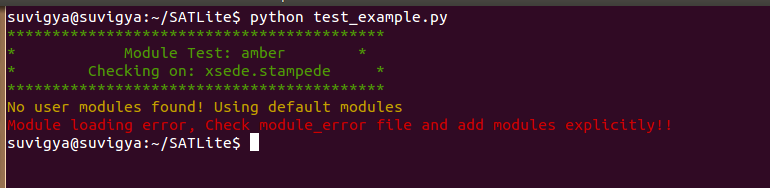
\includegraphics[width=16cm,height=4cm]{module_fail.png}
  \caption{Failure due to improper module loading}
  \label{fig:modfail}
  \end{center}
  \floatfoot{In Figure \ref{fig:modfail} execution failed as the modules required for the execution of Amber on Stampede had errors.}
\end{figure}

\begin{figure}
  \begin{center}
  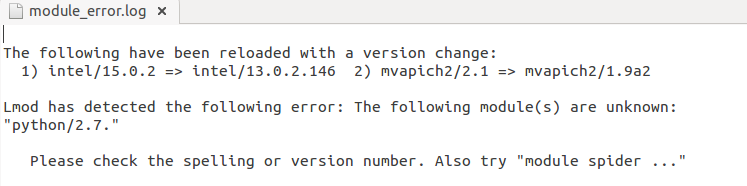
\includegraphics[width=18cm,height=5cm]{error1.png}
  \caption{Example of module\_error log file}
  \label{fig:log}
  \end{center}
  \floatfoot{Figure \ref{fig:log} shows an example of module\_error log file which provides explanation of possible error.}
\end{figure}

\begin{figure}
  \begin{center}
  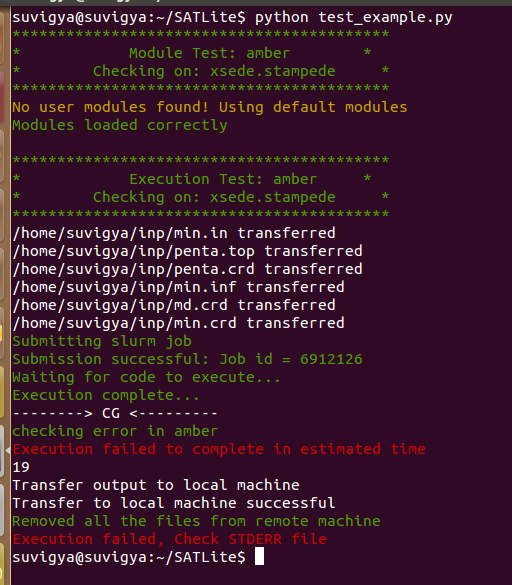
\includegraphics[width=15cm,height=16cm]{runtime.png}
  \caption{Execution failed to complete in the estimated time}
  \label{fig:runtimefail}
  \end{center}
  \floatfoot{In Figure \ref{fig:runtimefail}, the tool reported an error as the execution failed to complete in the estimated range provided by the user.}
\end{figure}

\begin{figure}
  \begin{center}
  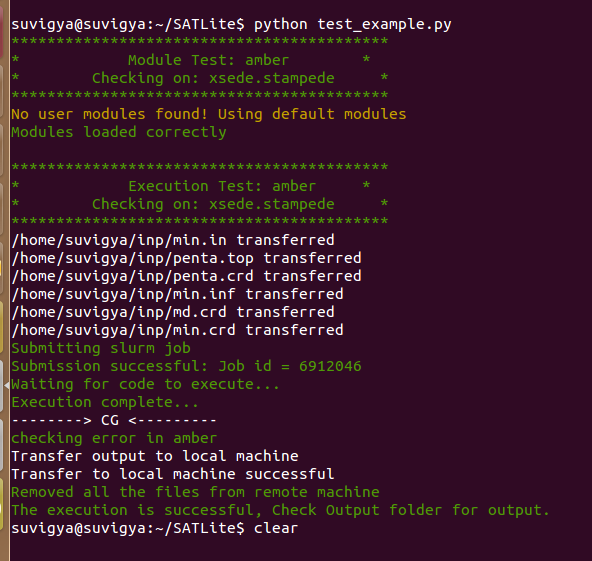
\includegraphics[width=15cm,height=16cm]{success.png}
  \caption{Successful Execution}
  \label{fig:success}
  \end{center}
  \floatfoot{In Figure \ref{fig:success}, tools reports successful execution as no errors or exceptions were reported during the execution.}
\end{figure}


\chapter{Continuous Integration}
Manual testing at times can be a laborious and time consuming process. Sometimes it is not feasible and efficient to test the same modules everytime if small change have been made. This difficulty further increases with the increase in complexity of components in a software product. Even if a single component change in such a complex and interdependent system can affect the behavior of other modules. This requires an urgency to implement an automated testing framework that can reduce manual testing work, simultaneously testing all of the critical components of the system. Continuous integration is a software engineering principle of rapid and automated development and testing. As discussed by Betz et al. \cite{ref16}, a continuous integration and central testing repository helps the developers to identify a broken test case or failure with certain compilers automatically whenever a change is pushed.

Testing is an inevitable part of any project and it is required to be automated and integral to build process so that developers do not have to manually test every aspect of their code. 

\section{About Continuous Integration}
The complete source code is required to be pushed on to central repository. GIT is the most common tool used for version control by recent day developers. Github provides online free code repository. Since, the major work done by the scientific community, especially Radical Group, is open source, Github becomes an obvious choice for controlling and maintaining our code repository. In a continuous integration life cycle, an automated system gets triggered when developers push their revised code on the repository. This system picks up the changes, pulls down the code and execute a few set of commands to verify that the application still works as expected even after the code modification \cite{ref17}. The most difficult part was to select the continuous integration server which would serve our purpose and execute our development stage unit cases for EnsembleMD and RepEx along with SATLite tool for testing deployment and run-time error reporting. The primary reasons for building an automated testing system are: 

\begin{itemize}
\item \textbf{Time saving:} Developers can save a considerable amount of time testing their build by automating the build and test phase.

\item \textbf{Improved software qualities:} Any detected issues can be resolved immediately, hence keeping software in a state where it can be safely released at any time.

\item \textbf{Faster development:} Development and release of any software is faster since manual integration issues are less likely to occur.
\end{itemize}


\section{Principles of Continuous Integration}

The software engineering practice of continuous integration was used to create a common build and test environment that integrates the developers’ code into one test environment and hence, errors can be detected on a commit basis \cite{ref26}. This section focuses on the main principles involved in the designing of continuous integration.

\subsubsection{\textbf{A. Maintain a Single Repository}}
One of the most important aspect of continuous integration is to maintain a single and central repository. This allows to keep track of multiple files and code changes. Maintaining a single repository can also prevent divergence in the code that could lead to difficult in resolving conflicts close to release. 

The current EnsembleMD and RepEx development process maintains a common Git repository for the source code. This feature has been extended to maintain a separate repository for the testing framework of the former tools.

\subsubsection{\textbf{B. Automate the Build}}
As projects gets larger and bigger, it becomes important that developers do not spend time in typing commands to compile, build and test the source code. The automated test build software ensures the efficiency and also allows for the easier support for many build options, such as building in virtual environment, execution on multiple supercomputers, etc.

\subsubsection{\textbf{C. Make the Build Self-testing}}
All software needs testing to eliminate source code bugs. Testing is a significant part of the software development cycle and validation needs to be automated and integral to the build process. The continuous integration is expected to build the code changes pushed to a central repository automatically and execute the testing suit to ensure that it behaves as expected by the developers. 

\subsubsection{\textbf{D. Frequent Commits}}
The practices of continuous integration encourages developers to commit their code changes as often as possible. This is beneficial to avoid merge conflicts if two developers are unknowingly modifying the same segment of the code. It is easier for the developers to merge, move, add or remove the code changes if the commits are more modular. Committing marks a point in the history of the code base where developers can switch back and use the changes made.

\subsubsection{\textbf{E. Testing in a Clone of Production Environment}}
It is highly likely that the production environment used by the end user is different from the development or the test environment. The testing environment should be close to the production environment. This principle aids in finding errors that may not be present on the developers' machine. 

\subsubsection{\textbf{F. Build and Test Result Availability}}
According to this principle, it is important to have a current development and staging build available at all times. Along with the build, the test result availability provides a visibility on the results to the developers.




\section{Selecting Continuous Integration Server}
The previous section discussed the principles and guidelines required to design a complete automated continuous integration server. There are a lot of existing and open source CI servers, namely, Jenkins \cite{site5}, GitLab \cite{site6}, Hudson, Cruise Control, TeamCity \cite{site7}, Travis, Cider \cite{ref18}, etc. Selecting the best and optimal CI server is the most arduous task. The most suitable continuous integration server should have certain features as discussed in table \ref{feature}. We have conducted a detailed study of the various available CI servers based on various features. Jenkins is Java based and is the most popular CI server which is compatible with most of the operating systems and a large number of languages. Moreover, it has multiple plug-ins to configure the required system-of-interest. Travis is also a commonly used CI server where each project runs in an individual virtual machine [23]. Testing open source projects in Travis is free of cost, but there is a charge for private repositories. TeamCity, developed by JetBrains, is an excellent paid CI server; whereas, Jenkins is a free open source server. TeamCity is extensively used in large organizations. GitLab is a more recent application which integrates source code management and a CI server, but it does not support as many plugins and languages as is supported by Jenkins \cite{ref16}, \cite{ref17}, \cite{ref20}. Table \ref{cicompare} summarizes and compares the different CI servers that were considered in the study.

\begin{table}
\begin{center}
\def\arraystretch{2}
\begin{tabular}{|p{1.5cm}|p{5cm}|p{8.5cm}|}
\hline
\rule{0pt}{15pt} \textbf{Sr No.} & \textbf{Feature} & \textbf{Remarks} \\[2ex]
\hline
1. & Version control system integration & CI system should support the integration with all the version control systems. \\
\hline

2. & First-time setup & CI system is expected to guide through the first time steps to setup the project.\\
\hline

3. & User Interface & CI system at minimum is expected to provide an overview of all the builds and allows to examine each specific build for more detailed information. \\
\hline

4. & Build Environment & CI system should supports large number of programming languages and has an extensive configuration properties. \\
\hline

5. & Feedback and reporting & CI systems should have mechanism to notify developers about the bugs or the issues.\\
\hline

6. & Post-build setups/ deployments & CI server should be able to deploy artifact to staging server, send emails, update bug, generate reports etc.\\
\hline

7. & Ease of extensibility & CI systems should be extensible and should provide large number of plug-ins.\\
\hline
\end{tabular}
\end{center}
\caption{Features of CI system}
\label{feature}
\end{table}


\begin{table}
\begin{center}
\def\arraystretch{2}
\begin{tabular}{|p{3cm}|p{3cm}|p{3cm}|p{3cm}|p{3cm}|}
\hline
\rule{0pt}{15pt} \textbf{Feature} & \textbf{Jenkins} & \textbf{Tavis} & \textbf{TeamCity} & \textbf{GitLab CI} \\[2ex]
\hline
Source availability model &  Free and Open Source & Free for open source project & Proprietary/ Closed source &  Free and Open source\\
\hline

Customizable and Scalable & Highly customizable. Large plugin ecosystem & Supports dozens of languages. & Supports large number of languages and APIs for extension. & Highly scalable. Tests can run on parallelly.\\
\hline

Operating System support & Supports Windows, Mac OS, Unix-like OS & OSX and Ubuntu. Windows not supported. Python not supported on OSX & Supported on Windows, Mac OS, Linux & Supported on Ubuntu, Debian, CentOS. Not supported on OSX, Windows, Fedora. \\
\hline

Integration & Can be integrated with all the source code management software. & Supports integration only with GitHub. &  Can be integrated with all the source code management software. & Officially integrates only with GitLab. \\
\hline

Tutorial and Documentation & Good tutorials available. Poor official documentation. &  Extensive and helpful documentation available. & Well documented. & Well documented.\\
\hline

Cost & Free & Not free for private repos & Expensive & Free \\
\hline

Capability & Easy installation, easy configuration, distributed builds, and extensive plugins. & Easy setup, multiple test environments for different runtime versions, helpful community. & Easy installation, great user interface. & Quick setup for the projects hosted on GitLab\\
\hline

\end{tabular}
\end{center}
\caption{Comparative study of CI servers}
\label{cicompare}
\end{table}

\begin{comment}
\begin{table}
\begin{center}
\def\arraystretch{2}
\begin{tabular}{|p{3.7cm}|p{3.7cm}|p{3.7cm}| p{3.7cm}|}
\hline
\rule{0pt}{15pt} \textbf{Jenkins} & \textbf{TeamCity} & \textbf{Hudson} & \textbf{Cruise Control} \\[2ex]
\hline
Jenkins's builds are made using an XML file. &
It supports build agents on different OS and based on different programming languages. &
Easy to setup and maintain. &
It is intended for Java and .Net applications.
\\
\hline
It has features like plugins, clear dashboard, code coverage, easy integration, new delivery of Jenkins job every week, post build tasks. &

\end{tabular}
\end{center}
\caption{Exposed SATLite tool APIs}
\label{cicompare}
\end{table}
\end{comment}

\section{Reasons to Select Jenkins}
The extensive research on which CI server serves our purpose has led us to choose Jenkins. Jenkins is very well established and extensively utilized CI server due to the following reasons:

\begin{itemize}
\item \textbf{Available Plugins:} Jenkins currently supports 392 plug-ins. It is a hub for the development of a large number of projects and applications due to it's powerful and diverse functionality.

\item \textbf{Cloud-enabled:} Cloudbees provides unlimited cloud space to the Jenkins users to build and test their code.

\item \textbf{Large number of developer:} Jenkins is maintained by a large number of developers who were initially members of the Hudson CI server. Since Jenkins has a team of well experienced developers, the software releases and upgrades are usually stable.
\end{itemize}

\section{Jenkins Integration}
Jenkins is the obvious choice for automated test bench integration of our development, deployment and run-time testing of EnsembleMD, RepEx and SATLite tool. Figure \ref{fig:jenkins_process} shows the stages in our Jenkins test process. The following are the generalized steps in integrating our testing with Jenkins:

\begin{figure}
  \begin{center}
  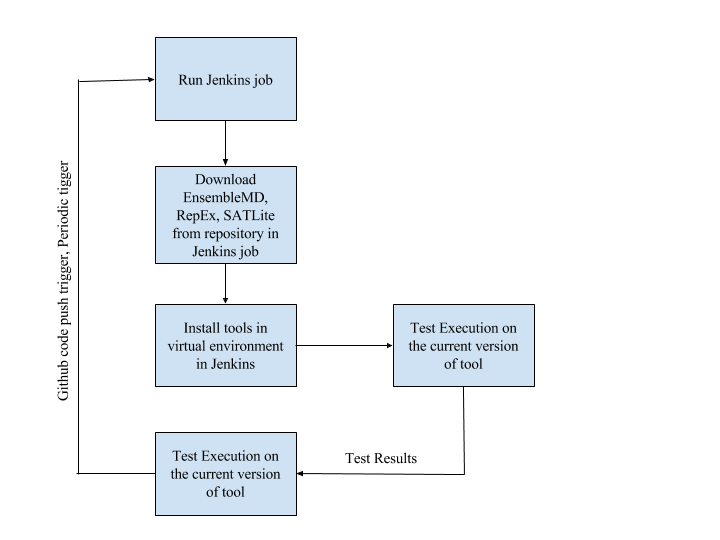
\includegraphics[width=13cm,height=9cm]{jenkins_process.png}
  \caption{Test Process using Jenkins}
  \label{fig:jenkins_process}
  \end{center}
\end{figure}

\begin{itemize}
\item Jenkins job gets triggered whenever changes are pushed into the Github repository or builds periodically even if the code base in not modified. This periodic build ensures that unmodified codes build and executes successfully on the remote machines.

\item Jenkins pulls the code from the tool repository and installs the tools in the virtual environment.

\item It then clones the test cases and executes unit test using py.test.

\item Post build generates a detailed test report showing the failure points, code coverage graphs, general trend in execution and violations in the python code formatting as shown in figures \ref{fig:test1},\ref{fig:failure_report}, \ref{fig:cov_table}. \ref{fig:cov_graph}, \ref{fig:trend}, \ref{fig:violation} and \ref{fig:vio_report}. 
\end{itemize}

\section{Post Build Actions}
After Jenkins build has finished execution and build, it generates different reports in order to provide detailed logging of the build. This section focuses on the various reporting mechanisms used in continuous integration system.

\subsubsection{\textbf{A. Test Case Report}}
Test case report provides a detailed result of the tests included in the build. It shows each test case function name with the failure or success report as shown in figure \ref{fig:test1}.

\begin{figure}
  \begin{center}
  %\begin{framed}
  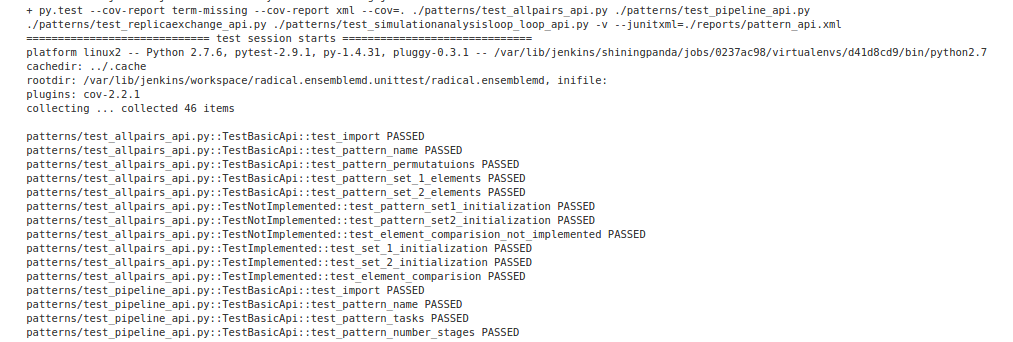
\includegraphics[width=17cm,height=6cm]{test1.png}
  %\end{framed}
  \caption{Each test case report}
  \label{fig:test1}
  \end{center}
\end{figure}


\subsubsection{\textbf{B. Failure Report}}
Jenkins exploits the characteristics of pytest that displays the possible reason for the failure. Figure \ref{fig:failure_report} shows an example of the detailed failure report. This is beneficial to debug the code bugs and resolve them.

\begin{figure}
 \begin{center}
 %\begin{framed}
  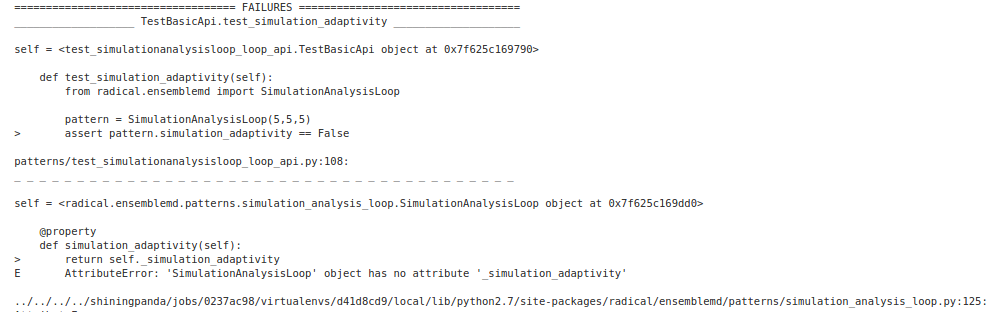
\includegraphics[width=15cm,height=5cm]{failure_report.png}
 % \end{framed}
  \caption{Example failure report}
  \label{fig:failure_report}
  \end{center}
\end{figure}


\subsubsection{\textbf{C. Code Coverage}}
Code coverage is a measure used to describe the extent of which the test code is tested by a test suit. A high code coverage shows that the program has been thoroughly tested and has lower chances of containing software bugs. Figure \ref{fig:cov_table} and Figure \ref{fig:cov_graph} shows code coverage in tabular and graphical format respectively.

\begin{figure}
 \begin{center}
 %\begin{framed}
  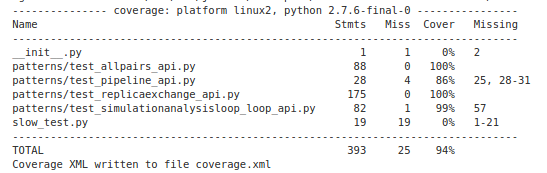
\includegraphics[width=15cm,height=5cm]{code_cov.png}
 % \end{framed}
  \caption{Code Coverage: Tabular format}
  \label{fig:cov_table}
  \end{center}
\end{figure}


\begin{figure}
 \begin{center}
 %\begin{framed}
  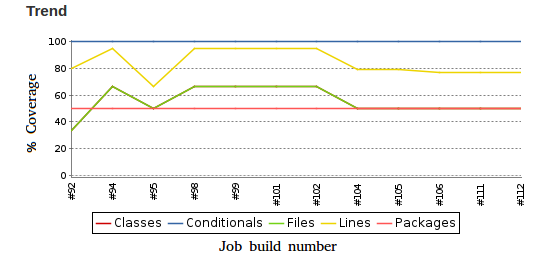
\includegraphics[width=15cm,height=7cm]{cov_graph.png}
 % \end{framed}
  \caption{Code Coverage: Graphical format}
  \label{fig:cov_graph}
  \end{center}
\end{figure}

\begin{comment}
\begin{figure}
\centering
\begin{subfigure}{.5\textwidth}
  \centering
  %\begin{framed}
  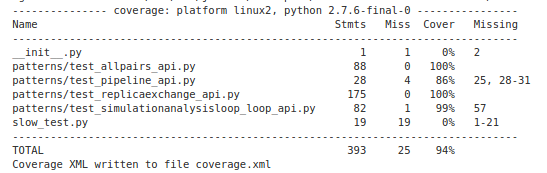
\includegraphics[width=8cm,height=3cm]{code_cov.png}
  %\end{framed}
  \caption{Tabular format}
  \label{fig:cov_table}
\end{subfigure}%
\begin{subfigure}{.5\textwidth}
  \centering
  %\begin{framed}
  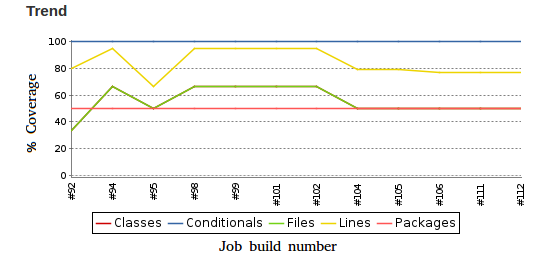
\includegraphics[width=8cm,height=5cm]{cov_graph.png}
  %\end{framed}
  \caption{Graphical format}
  \label{fig:cov_graph}
\end{subfigure}
\caption{Code Coverage}
\label{fig:cov}
\end{figure}
\end{comment}


\subsubsection{\textbf{D. Trend Graph}}
Trend Graph shows a general trend of success and failures of the builds. The greater the red area, the greater the failure. This type of graph provides a visual effect of the success ratio of the builds. Figure \ref{fig:trend} shows an example of a success-failure trend.

\label{}
\begin{figure}
 \begin{center}
  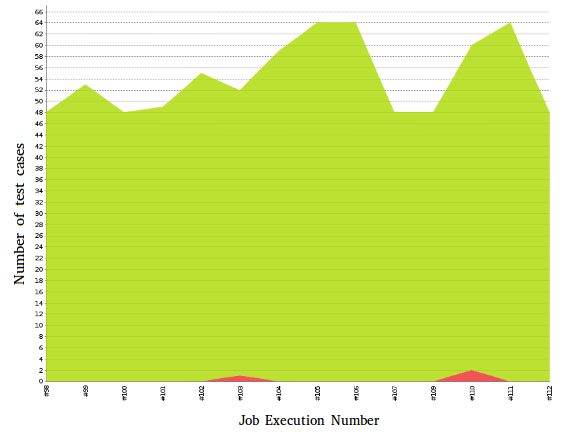
\includegraphics[width=15cm,height=7cm]{trends.png}
  \caption{Success-Failure trend graph}
  \label{fig:trend}
  \end{center}
\end{figure}

\subsubsection{\textbf{E. Code Format}}
Code formatting of any specific language should be ubiquitous. A properly formatted code is easy to distribute, understand and is universally accepted. Our continuous integration system uses pylint to check the python code formatting using standard PEP 8 (Style Guide for Python Code). Pylint checks the code-line length, checks for proper spacing, checks if imported modules are used, etc. Figure \ref{fig:violation} shows the graphical view of violations in the code formatting. The red section in the graph represents a higher priority of violations which needs to be resolved before any product release. Medium and Low violations have less priority and can be ignored as they include unused modules or spacing issues. Figure \ref{fig:vio_report} shows an example of the detailed report of the violations with low, medium and high priorities. The report also shows the exact location and reason for the violation.

\label{}
\begin{figure}
 \begin{center}
  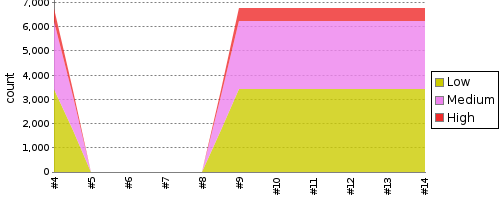
\includegraphics[width=15cm,height=6cm]{violation.png}
  \caption{Code Format Violations}
  \label{fig:violation}
  \end{center}
\end{figure}

\label{}
\begin{figure}
 \begin{center}
  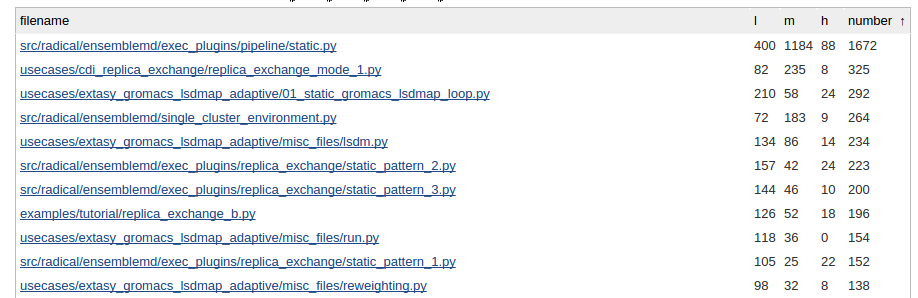
\includegraphics[width=17cm,height=6cm]{vio_report.png}
  \caption{Code Format Violation Report}
  \label{fig:vio_report}
  \end{center}
\end{figure}


\begin{table}
\begin{center}
\def\arraystretch{2}
\begin{tabular}{|p{2.5cm}|p{8cm}|p{5cm}|}
\hline
\rule{0pt}{5pt} \textbf{Application} & \textbf{Command} & \textbf{Remarks} \\[2ex]
\hline
Amber & python satlite\_exe.py --name ``amber" --resource ``xsede.stampede" --arguments amber\_arguments.wcfg & Single executable example. Tested on Stampede.
\\
\hline
CoCo & python satlite\_exe.py --name ``coco" --resource ``xsede.stampede" --arguments coco\_arguments.wcfg & Single executable example. Tested on Stampede.
\\
\hline
Gromacs & python satlite\_exe.py --name ``gromacs" --resource ``xsede.stampede" --arguments gromacs\_arguments.wcfg & Single executable example. Tested on Stampede.
\\
\hline
LSDMap & python satlite\_exe.py --name ``lsdmap" --resource ``xsede.stampede" --arguments lsdmap\_arguments.wcfg & Single executable example. Tested on Stampede.
\\
\hline
Hello World & python satlite\_exe.py --name hello --resource xsede.stampede --exe {``icpc",``ibrun"} --arguments {``hello\_test1.wcfg",``hello\_test2.wcfg"} & Hello world example with multiple executable. Two executable for compiling and executing c++ hello world program. Tested on Stampede.
\\
\hline
\end{tabular}
\end{center}
\caption{Example of SATLite testing scientific tool}
\label{satexample}
\end{table}

\chapter{Conclusion and Future Work}

\section{Conclusion}
In this thesis, we attempted to address the issue of HPC resource wastage by minimizing the errors right from the development phase of an application. This thesis pivots around the errors in the on-going development of scientific tools especially molecular dynamics packages and simulations such as Amber, CoCo, LSDMap and Gromacs. It also provides a continuous testing framework to test EnsembleMD toolkit and RepEx frameworks which serves as an abstraction tool for MD simulation packages. The intensive study for this thesis focuses on setting up a 3-stage automatic testing and error reporting framework, the three stages being development, deployment and run-time. As reported by several researchers, a large amount of HPC resource is wasted due to system failures. Their studies mainly concentrated on techniques to curtail the errors from a supercomputers' perspective. The study in this thesis provides a solution to combat the errors at the application level. Mining and analyzing the system logs is universal approach to develop tool that can automatically detect the error and generate failure reports with proper justification. Although, Oliner et al. \cite{ref14} discusses that the logs from the supercomputers does not provide sufficient information to perform automatic detection of failures. Moreover, the system logs does not provide a real-time status of the application. We have used console logs to detect various parameters such as job id or errors or exit codes.

The unit testing and end-to-end testing for EnsembleMD and RepEx covered the important APIs and functionalities to check the software and implementation bugs. These toolkits were continuously tested by Jenkins CI server, hence ensuring their stability. We observed that the test cases we developed could successfully test the proper functioning of EnsembleMD and RepEx and capture the errors in the source code. The development level testing can help in fixing the software bugs right in the development phase. The SATLite tool was able to capture deployment and run-time errors when scientific tools are executed directly on to the supercomputers. This error reporting can help molecular dynamics community and developers to achieve confidence in their simulation packages. We were able to capture environment setup failures, errors due to obsolete modules, input file errors, execution failures or even improper execution. 

\section{Future Work}
There is a broad scope in the development of error detection tools to enhance the performance of applications on supercomputing resources. An ideal bug-free application should be tolerant to any system upgrades or changes and should have optimized execution to utilize maximum performance of supercomputers. As the scientific tools are continuously updating so are EnsembleMD and RepEx. There is always an opportunity to increase the number of test scenarios to check the source code bugs and to establish a confidence in the application. 

The SATLite tool has been currently developed for SLURM job schedulers and tested on Stampede supercomputer. In future scope, SATLite has to be extended for resources with other job schedular such as PBS. To achieve this, one of the approach could be to use Radical SAGA \cite{ref23},\cite{site9} as an underlying framework as it can handle large number of job schedulers and batch scripts. Moreover, error detection can be improved by translating exit code to text based reporting. A more intensive usage of SATLite with large number of scientific applications can help in expanding this testing framework. The proof-of-concept of SATLite proves to be promising in minimizing the application failures due to software bugs or improper environment loading or incorrect input files. It can be used by the developers and scientists to scrutinize their application before actually releasing it for their users.

\section{Links to Current Work}
The current development version of the testing framework can be downloaded from the below mentioned Github links.

\begin{itemize}
\item \textbf{EnsembleMD Unit Testing:} https://github.com/suvigya91/EnsembleMD-Testsuit

\item \textbf{RepEx Unit Testing:} https://github.com/suvigya91/repex-test

\item \textbf{SATLite- Deployment and Run-time testing suit:} https://github.com/suvigya91/SATLite

\item \textbf{SATLite readthedocs:} http://satlite.readthedocs.io/en/latest/
\end{itemize}
%\input{}

% R E F E R E N C E S
\def\aap{{A\&A}}
\def\aas{{A\&AS}}
\def\aj{{AJ}}
\def\araa{{ARA\&A}}
\def\apj{{ApJ}}
\def\apjl{{ApJ}}
\def\apjs{{ApJS}}
\def\baas{{BAAS}}
\def\mnras{{MNRAS}}
\def\nat{{Nature}}
\def\pasp{{PASP}}

\clearpage
\addcontentsline{toc}{chapter}{References}
\bibliographystyle{apj}
\bibliography{thesis}

\renewcommand{\bibname}{References}

\begin{thebibliography}{30}

\bibitem{ref1}
Mary Qu Yang, Jack Y. Yang.
\textit{High-Performance Computing for Drug Design.}
In Bioinformatics and Biomedicine Workshops, 2008 IEEE Conference,
Philadelphia, PA.

\bibitem{ref2}
Vivekanandan Balasubramanian, Antons Treikalis, Ole Weidner, Shantenu Jha.
\textit{EnsembleMD Toolkit: Scalable and Flexible Execution of Ensembles of Molecular Simulations}, 2016 Cornell University Library, arXiv:1602.00678v2.

\bibitem{ref3}
Vivekanandan Balasubramanian.
\textit{Towards Frameworks for Large Scale Ensemble-based Execution Patterns}.
In Master's thesis, 2015 Rutgers University.

\bibitem{ref4}
Yugi Sugita, Yuko Okamoto.
\textit{Replica-exchange molecular dynamics method for protein folding}.
In Chemical Physics Letters, Volume 314, Issues 1–2, 26 November 1999, Pages 141–151.

\bibitem{ref5}
Antons Treikalis, Andre Merzky, Haoyuan Chen, Tai-Sung Lee, Darrin M. York, Shantenu Jha.
\textit{RepEx: A Flexible Framework for Scalable Replica Exchange Molecular Dynamics Simulations}, 2016 Cornell University Library, arXiv:1601.05439v1.

\bibitem{ref6}
Catello Di Martino, Zbigniew Kalbarczyk, William Kramer, Ravishankar Iyer.
\textit{Measuring and Understanding Extreme-Scale Application Resilience: A Field Study of 5,000,000 HPC Application Runs}.
In Proceedings of 45th Annual IEEE Conference Dependable Systems and Networks, 2015, IEEE Computer Society.

\bibitem{ref7}
Eric Heien, Derrick Kondo, Ana Gainaru, Dan LaPine, Bill Kramer, Frank Cappello.
\textit{Modeling and Tolerating Heterogeneous Failures in Large Parallel Systems}.
In 2011 ACM, Seattle, Washington.

\bibitem{ref8}
Bianca Schroeder, Garth A. Gibson.
\textit{A Large-Scale Study of Failures in High-Performance Computing Systems}.
Proceedings in IEEE Transactions on Dependable and Secure Computing, IEEE Computer Society, 2010.

\bibitem{ref9}
Edward Chuah, Shyh-hao Kuo, Paul Hiew, William-Chandra Tjhi, Gary Lee, John Hammond, Marek T. Michalewicz, Terence Hung, James C. Browne.
\textit{Diagnosing the Root-Causes of Failures from Cluster Log Files}, 
Proceeding from International Conference on High Performance Computing, 2010 IEEE.

\bibitem{ref10}
Xin Chen, Charng-Da Lu, Karthik Pattabiraman.
\textit{Predicting Job Completion Times Using Systems Logs in Supercomputing Clusters}.
Proceedings of 43rd Annual IEEE/IFIP Conference.
Dependable Systems and Networks Workshop (DSN-W), 2013.

\bibitem{ref11}
Sean R Eddy.
\textit{Hidden Markov models}.
In Current Opinion in Structural Biology, 
Volume 6, Issue 3, June 1996, Pages 361–365.

\bibitem{ref12}
Ana Gainaru, Franck Cappello, Marc Snir, William Kramer.
\textit{Fault Prediction under the microscope: A closer look into HPC systems}.
Proceeding of International Conference for High Performance Computing, Networking, Storage and Analysis (SC), 2012 IEEE. Pages 1-11, Salt Lake City, UT.

\bibitem{ref13}
\textit{Towards Increasing the Error Handling Time Window in Large-Scale Distribured Systems using Console and Resource Usage Logs}.
Proceeding of IEEE Conference on Trustcom, BigDataSE and ISPA, 2015 (Vol 3),
Helsinki. Pages 61-68.

\bibitem{ref14}
Adam Oliner, Jon Stearley.
\textit{What Supercomputers Say: A Study of Five System Logs}.
Proceeding of 37th Annual IEEE/IFIP International Conference on Dependable Systems and Networks (DSN'07), 2007 IEEE, Edinburgh. Pages 575-584.

\bibitem{ref15}
Gengbin Zheng, Lixia Shi, Laxmikant V. Kale.
\textit{FTC-Charm++: An In-Memory Checkpoint-Based Fault Tolerant Runtime for Charm++ and MPI}.
Proceedig of International Conference on Cluster Computing, 2004, IEEE. 
Page 93-103.

\bibitem{ref16}
Robin M. Betz, Ross C. Walker.
\textit{Implementing Continuous Integration Software in an Established Computional Chemistry Software Package}.
Proceeding of 5th International Workshop on Software Engineering for Computational Science and Engineering (SE-CSE), 2013 IEEE, San Francisco. Page 68-74.

\bibitem{ref17}
Mathias Meyer.
\textit{Continuous Integration and Its Tools}.
In IEEE Software (Vol 31, Issue 3), Sponsored by IEEE Computer Society.
Page 14-16.

\bibitem{ref18}
Ondrej Kupka, Filip Zavoral.
\textit{Cider: An Event-driven Continuous Integration Server}.
Proceeding of Computer Software and Applications Conference (COMPSAC), 2014 IEEE 38th Annual Conference, Vasteras. 
Page 646-647

\bibitem{ref19}
Leonard Bautista-Gomez, Anne Benoit, Aurelien Cavelan, Saurabh K. Raina, Yves Robert, Hongyan Sun.
\textit{Which Verification for Soft Error Detection}.
Proceeding of 22nd International Conference on High Performance Computing (HiPC), 2015 IEEE, Bangalore. Page 2-11

\bibitem{ref26}
Robin M. Betz, Ross C. Walker.
\textit{Implementing Continuous Integration Software in an Established Computational Chemistry Software Package}.
Proceedings of the 5th International Workshop on Software Engineering for Computational Science and Engineering, 2013 ACM.

\bibitem{ref20}
Preeti Rai, Madhurima, Saru Dhir, Madhulika, Anchal Garg.
\textit{A Prologue of Jenkins with Comparative Scrutiny of Various Software Integration Tools}.
Proceedings of 2nd International Conference on Computing for Sustainable Global Development (INDIACom), 2015 IEEE, New Delhi. Page 201-205.

\bibitem{ref21}
Mohammad Wahid, Abdullah Almalaise.
\textit{JUnit Framework: An Interactive Approach for Basic Unit Testing Learning in Software Engineering}.
Proceedings of 3rd International Congress on Engineering Education (ICEED), 2013 IEEE, Kuala Lumpur. Page 159-164.

\bibitem{ref22}
Andre Merzky, Mark Santcroos, Matteo Turilli, Shantenu Jha.
\textit{RADICAL-Pilot: Scalable Execution of Heterogeneous and Dynamic Workloads on
Supercomputers}.
2015 Cornell University Library.

\bibitem{ref23}
Andre Luckow, Lukas Lacinski, Shantenu Jha 
\textit{SAGA BigJob: An Extensible and Interoperable Pilot-Job Abstraction for Distributed Applications and Systems}.
In proceeding of Symposium on Cluster, Cloud and Grid Computing, 2010 10th IEEE/ACM International, Melbourne. Page 135 - 144.

\bibitem{ref24}
Harsh Bhasin, Esha Khanna, Sudha.
\textit{Black Box Testing based on Requirement Analysis and Design Specifications}.
2014, International Journal of Computer Applications (0975 – 8887), Vol 87 -No.18.

\bibitem{ref25}
Srinivas Nidhra, Jagruthi Dondeti.
\textit{Black box and White box Testing Techniques: A Literature Review}.
In International Journal of Embedded Systems and Applications (IJESA) Vol.2, No.2, June 2012.

\bibitem{site1}
Radical EnsembleMD Readthedocs.
http://radicalensemblemd.readthedocs.io/en/master/index.html

\bibitem{site2}
Radical RepEx Readthedocs.
http://repex.readthedocs.io/en/latest/

\bibitem{site3}
Radical Pilot Readthedocs.
https://radicalpilot.readthedocs.io/en/stable/

\bibitem{site9}
Radical SAGA.
http://saga-python.readthedocs.io/en/latest/

\bibitem{site4}
Continuous Integration With Gitlab CI. http://alanmonger.co.uk/php/continuous/integration
/gitlab/ci/docker/2015/08/13/continuous-integration-with-gitlab-ci.html

\bibitem{site5}
Jenkins CI server.
https://jenkins.io/

\bibitem{site6}
GitLab CI server.
https://about.gitlab.com/

\bibitem{site7}
TeamCity CI server
https://www.jetbrains.com/teamcity/

\bibitem{site8}
BuildForge CI server.
http://www.ibm.com/developerworks/downloads/r/rbuildforge/

\bibitem{site10}
Static Testing.
http://www.tutorialspoint.com/software\_testing\_dictionary/static\_testing.htm


\end{thebibliography}
% A P P E N D I X
\appendix

%\input{pca_appendix}

\clearpage

\pagestyle{empty}
%\input{vita}

\end{document}

